\documentclass[11pt,a4paper]{article}
\pdfinfoomitdate=1
\pdftrailerid{}
\pdfsuppressptexinfo=15
\usepackage[T1]{fontenc}
\usepackage{lmodern}
\usepackage[margin=1.05in]{geometry}
\usepackage{amsmath,amssymb,amsthm,mathtools}
\usepackage{graphicx,booktabs,array,microtype}
\usepackage{tikz}
\usetikzlibrary{arrows.meta,calc,patterns,positioning,decorations.pathreplacing}
\usepackage[dvipsnames]{xcolor}
\usepackage[colorlinks=true,linkcolor=MidnightBlue,citecolor=MidnightBlue,urlcolor=MidnightBlue]{hyperref}
\hypersetup{pdftitle={Quenched SLE3 limits for general weak random-bond Ising models},pdfauthor={OpenAI},pdfsubject={Critical interfaces with bounded independent disorder}}
\numberwithin{equation}{section}
\newtheorem{theorem}{Theorem}[section]
\newtheorem{proposition}[theorem]{Proposition}
\newtheorem{lemma}[theorem]{Lemma}
\newtheorem{corollary}[theorem]{Corollary}
\theoremstyle{definition}
\newtheorem{definition}[theorem]{Definition}
\theoremstyle{remark}
\newtheorem{remark}[theorem]{Remark}
\newcommand{\E}{\mathbb E}
\newcommand{\Prob}{\mathbb P}
\newcommand{\R}{\mathbb R}
\newcommand{\C}{\mathbb C}
\newcommand{\Z}{\mathbb Z}
\newcommand{\N}{\mathbb N}
\newcommand{\1}{\mathbf 1}
\newcommand{\dd}{\mathrm d}
\DeclareMathOperator{\Cov}{Cov}
\DeclareMathOperator{\Var}{Var}
\DeclareMathOperator{\diam}{diam}
\DeclareMathOperator{\dist}{dist}
\DeclareMathOperator{\supp}{supp}
\DeclareMathOperator{\osc}{osc}
\DeclareMathOperator{\TV}{TV}
\DeclareMathOperator{\SLE}{SLE}
\setlength{\emergencystretch}{2em}
\setcounter{tocdepth}{2}
\title{Quenched $\mathrm{SLE}_3$ limits for general\\ weak random-bond Ising models}
\author{OpenAI}
\date{October 5, 2026}
\begin{document}
\maketitle
\begin{abstract}
For the planar Ising model with bonds $J_e=1+\varepsilon\xi_e$, where the
$\xi_e$ have any fixed bounded, nondegenerate, mean-zero iid law, we prove
quenched chordal $\mathrm{SLE}_3$ convergence for sufficiently small
$\varepsilon>0$. The temperature is the spontaneous-magnetization threshold.
Convergence holds in probability over environments for the full oriented
curve law in deterministic Jordan-domain approximations.
\end{abstract}
\tableofcontents
\section{Introduction}\label{sec:introduction}

The critical planar Ising model has a conformally invariant interface limit.
For a random ferromagnet, the corresponding question asks whether weak
microscopic disorder disappears from the macroscopic law when the environment
is held fixed. In two dimensions the disorder is marginal, so a scale-by-scale
decay estimate is needed in place of a uniform contraction.
We extend the weak symmetric two-valued result of~\cite{R} to general
bounded iid bond laws. The law need not be preserved by planar duality,
so the proof must identify the critical temperature without assuming
distributional self-duality.

\subsection{Model and statement}
Let $\rho$ be a probability measure supported on $[-1,1]$ such that
\begin{equation}\label{eq:law-assumptions}
 \int x\,\rho(\dd x)=0,
 \qquad \sigma_\rho^2:=\int x^2\,\rho(\dd x)>0.
\end{equation}
On the unoriented nearest-neighbor edges of $\Z^2$, let $(\xi_e)_e$ be
independent with law $\rho$, and set
\begin{equation}\label{eq:bond-model}
 J_e=1+\varepsilon\xi_e,\qquad 0<\varepsilon<1.
\end{equation}
Write $\omega=(\xi_e)_e$ for the environment and $\Prob_\rho$ for its product
law. For a finite spin domain $\Lambda$, inverse temperature $\beta\geq0$,
and prescribed exterior spins $\tau$, the quenched Ising law has weight
\[
 \exp\!\left(\beta\sum_{\{x,y\}:\{x,y\}\cap\Lambda\ne\varnothing}
       J_{\{x,y\}}\sigma_x\sigma_y\right),
 \qquad \sigma_x=\tau_x\quad(x\notin\Lambda),
\]
where the sum runs over nearest-neighbor edges with at least one free endpoint.
Expectations for this law are denoted by $\langle\,\cdot\,\rangle^\tau_{
\Lambda,\beta,J}$. Put $B_m=[-m,m]^2\cap\Z^2$ and define
\begin{equation}\label{eq:critical-definition}
 \beta_c^\rho(\varepsilon)
 =\inf\left\{\beta\geq0:
 \E_\rho\!\left[\lim_{m\to\infty}
       \langle\sigma_0\rangle^+_{B_m,\beta,J}\right]>0\right\}.
\end{equation}
The plus-state limit exists by ferromagnetic monotonicity. Throughout the
paper, averaging a quenched law means integrating it against $\Prob_\rho$;
the environment is never reweighted by a partition function.
We write $K_0=\tfrac12\log(1+\sqrt2)$ for the pure critical coupling.

Let $D\subset\C$ be a bounded Jordan domain with distinct marked boundary
points $a,b$. A lattice approximation is a simply connected square-lattice domain
containing every interior nearest-neighbor bond, embedded with mesh
$\delta$, with a Jordan boundary and marked interface endpoints
$a_\delta,b_\delta$. We call such a domain full. The boundary approximation used
here means that there are homeomorphisms
\begin{equation}\label{eq:boundary-approximation}
 h_n:\partial D\longrightarrow\partial D_n,
 \qquad \sup_{z\in\partial D}|h_n(z)-z|\longrightarrow0,
 \qquad (a_n,b_n)\longrightarrow(a,b).
\end{equation}
The graphs and bond variables live on the unit lattice and are then embedded
by multiplication by $\delta_n$. This convention allows all $n$ to use one
environment. The exterior-neighbor and pinned-boundary-vertex conventions are specified
in Section~\ref{sec:interface}.

Dobrushin conditions fix plus spins on one marked arc and minus spins on
the other. The arc assignments must give a consistent spin at every
pinned site. The spin interface is oriented from $a_n$ to $b_n$ and uses the
deterministic north-east/south-west pairing whenever a contour vertex has
degree four. We use continuous polygonal representatives of the resulting
oriented curves. For two such curves, let
\begin{equation}\label{eq:curve-metric}
 d_{\rm curv}(\gamma,\eta)
   =\inf_{\phi,\psi}\sup_{t\in[0,1]}
          |\gamma(\phi(t))-\eta(\psi(t))|,
 \qquad \bar d_{\rm curv}=1\wedge d_{\rm curv},
\end{equation}
where $\phi,\psi$ range over increasing homeomorphisms of $[0,1]$; curves
at zero distance are identified. For probability laws on this space, set
\begin{equation}\label{eq:BL-definition}
 d_{\rm BL}(\mu,\nu)
 =\sup\left\{\left|\int F\,\dd\mu-\int F\,\dd\nu\right|:
       \|F\|_\infty\leq1,\ 
       |F(\gamma)-F(\eta)|\leq\bar d_{\rm curv}(\gamma,\eta)\right\}.
\end{equation}
This is a bounded-Lipschitz metric for weak convergence in the oriented
uniform-curve topology. Write $Q_{n,\omega}$ for the quenched Dobrushin
interface law and $\mathsf S_{D;a,b}$ for chordal $\SLE_3(D;a,b)$.

\begin{theorem}\label{thm:main}
For every law $\rho$ satisfying \eqref{eq:law-assumptions}, there exists
$\varepsilon_0(\rho)>0$ with the following property. Fix
$0<\varepsilon<\min\{1,\varepsilon_0(\rho)\}$. For every bounded Jordan
domain $D$, distinct $a,b\in\partial D$, and deterministic square-lattice
approximations satisfying \eqref{eq:boundary-approximation} with
$\delta_n\downarrow0$, the interface law at
$\beta=\beta_c^\rho(\varepsilon)$ satisfies
\begin{equation}\label{eq:main-convergence}
 d_{\rm BL}(Q_{n,\omega},\mathsf S_{D;a,b})
     \xrightarrow[n\to\infty]{\Prob_\rho}0.
\end{equation}
The disorder threshold depends on $\rho$ and not on $D$, its marked points,
or the approximation sequence. Moreover,
$\beta_c^\rho(\varepsilon)=\tfrac12\log(1+\sqrt2)+O_\rho(\varepsilon^2)$.
\end{theorem}

\subsection{History and relation to earlier work}
The effect of weak bond disorder is especially delicate in two dimensions.
Harris's relevance criterion places the pure Ising model at the marginal
case, where the specific-heat exponent is zero and the criterion alone
does not decide the effect of randomness~\cite{Harris}.
Dotsenko and Dotsenko's fermionic analysis predicted a double logarithmic
specific-heat singularity~\cite{DD,DDReview}. Renormalization-group work
of Jug, Shalaev, Shankar, and Ludwig developed and refined the description
of logarithmic corrections to pure-model critical behavior
\cite{Jug,Shalaev,Shankar,Ludwig}. The predictions for different correlation
observables were not identical throughout this development. The relevant
physical picture here is marginal irrelevance: weak disorder decreases
under changes of scale, but only logarithmically. These works concern
thermodynamic quantities and correlations; control of a quenched law for
an entire interface also requires geometric estimates.

For the homogeneous critical model, the conformal description is
rigorous. Schramm's stochastic Loewner evolution supplies the candidate
interface laws~\cite{Schramm}. Smirnov established conformal convergence
of the FK-Ising fermionic observable~\cite{Smirnov}, and Chelkak and
Smirnov proved fermionic-observable universality for critical isoradial
Ising models~\cite{ChelkakSmirnov}. Chelkak, Duminil-Copin, Hongler,
Kemppainen, and Smirnov proved that the critical square-lattice spin
interface with Dobrushin boundary conditions converges to chordal
$\mathrm{SLE}_3$ in uniform distance modulo increasing
reparametrization~\cite[Theorem~1 and Equation~(1)]{CDHKS}.
This is the pure interface theorem underlying our comparison argument.

Rigorous universality results for deterministic interactions provide a
second point of comparison. Giuliani, Greenblatt, and Mastropietro proved
universality of infinite-plane energy-correlation scaling limits for
weak finite-range pair perturbations with lattice symmetries
\cite[Theorems~1.1--1.2]{GGM}. For non-integrable spin interfaces,
Greenblatt and Peltola constructed a Grassmann representation of a
discrete martingale and formulated the correlation estimates needed for
a proposed route to $\mathrm{SLE}_3$
\cite[Theorem~4.4 and Conjecture~4.5]{GP}. Their paper does not prove
interface convergence. For random bonds, Mahfouf proved quenched
FK-interface convergence to $\mathrm{SLE}_{16/3}$ in a regime where the
disorder strength tends to zero with the mesh
\cite[Theorem~1.6]{Mahfouf}. Av\'erous and Mahfouf established
high-probability crossing estimates for near-critical random-bond
FK models, also with vanishing disorder for $1<q\le4$
\cite[Theorems~1.5--1.6]{AM}. In the present theorem the nonzero disorder
strength is fixed as the mesh tends to zero, and the interface separates
spin clusters.

The main theorem of~\cite{R} treats symmetric two-valued bond disorder,
whereas its local scale transformation, moment estimates, and marginal
variance estimate are formulated for more general random local potentials.
We verify their hypotheses for the law~$\rho$ and its exact dual, and use
the pure and deterministic boundary-comparison results of~\cite{S}
through their formulations in~\cite{R}. The critical-point argument
adapts the torus method of~\cite[Section~8]{R} to match two separately
tuned trajectories within the same physical temperature family.
This matching replaces distributional self-duality.

Duality has a substantial history in the study of disordered critical
points. Chayes and Shtengel established vanishing magnetization and
critical correlation properties for self-dual disordered ferromagnets
under their stated hypotheses~\cite[Theorems~$1'$--$2'$]{ChayesShtengel}.
Our general one-edge law need not be self-dual. We use Kramers--Wannier
duality~\cite{KW} in the finite-torus form of Bugrij and Shadura, which
relates the four periodic/antiperiodic partition functions for arbitrary
positive inhomogeneous couplings~\cite[Equations~(4)--(5)]{BS}.
The torus comparison identifies the two tuned temperatures; a separate
argument identifies their common value with the spontaneous-magnetization
threshold.

The remaining argument combines classical probabilistic tools with
the geometric inputs of~\cite{R,S}. The Fortuin--Kasteleyn representation~\cite{FK}, the
Edwards--Sokal coupling~\cite{ES}, and the FKG lattice
inequality~\cite{FKG} relate spin barriers, random-cluster connections,
and boundary monotonicity. The decision-tree inequality of O'Donnell,
Saks, Schramm, and Servedio~\cite{OSSS}, extended to monotonic measures
by Duminil-Copin, Raoufi, and Tassion~\cite[Theorem~1.1]{DCRT}, is
applied at each fixed environment before averaging over the bonds.
The geometric use of crossing estimates to control random curves has
precedents in Aizenman--Burchard~\cite{AB} and
Kemppainen--Smirnov~\cite{KS}; Sheffield--Sun~\cite{SS} distinguish
convergence of driving functions from convergence in the uniform curve
topology. The specific passage from boundary barriers and trace
convergence to oriented-curve convergence used here is the progress
criterion of~\cite[Section~9]{R}.


\subsection{The extension and the proof}
The local scale transformation of~\cite{R} rewrites the model as a
sequence of random local perturbations of pure critical Ising.
Section~\ref{sec:scale} states the analytic estimates, and
Section~\ref{sec:tuning} verifies their hypotheses for the primal and
exact dual families and chooses a temperature for each at which the
perturbations tend to zero in environmental moments. The variance coordinate retains local cubic
terms, so the estimates also cover laws with nonzero third moment.

The two families are parametrized by the same physical inverse
temperature, but their selected temperatures need not initially agree.
Section~\ref{sec:matching} compares the four torus partition functions
along these trajectories. Exact duality shows that, at both selected
temperatures, the same primal FK winding event has probability
asymptotic to its pure critical probability. Monotonicity and a quantitative
lower bound for its temperature derivative then force the temperatures to
agree. This identifies a common primal-dual temperature without
assuming symmetry of the disorder law.

Section~\ref{sec:crossings} transfers the decaying perturbations to local
conditional crossing estimates and joint laws of finitely many crossing
tests on tori. The error
terms are geometrically weighted; decay suffices even though the scale
norms need not be summable. Section~\ref{sec:criticality} uses the
estimates on both lattices to identify the common temperature with
\eqref{eq:critical-definition}. Barriers in annuli with disjoint bond
neighborhoods first rule out percolation there. Above that temperature,
an environmental amplification argument and the decision-tree inequality
give rapid dual-arm decay and positive primal magnetization.

Section~\ref{sec:interface} uses the boundary-comparison results
of~\cite{R,S} to compare the random interface with pure interfaces in
slightly displaced domains. The couplings retain the pure comparison
law conditional on the original environment. This conditional marginal
turns the comparison into a quenched statement. A planar sandwich
identifies the trace, and a separate multi-passage estimate controls
its order of traversal, giving the full metric
in~\eqref{eq:curve-metric}.

\section{Scale estimates for general local arrays}
\label{sec:scale}

We first state the scale estimates that will be used to choose the
temperature.  These are results about local random potentials, rather
than about a particular one-edge distribution.  We use the exact energy
charge, local transformation, moment estimates, and variance coordinate
of \cite[Sections~2--5]{R}.  The hypotheses below explain why those
results apply to the present law \(\rho\), although the main theorem of
\cite{R} concerns symmetric two-valued disorder.  The pure-model inputs
behind that construction are developed in \cite[Sections~2--3]{S}.

\subsection{The reference field and its energy charge}

Let \(\E_0\) denote expectation under the full-plane critical Ising
law at \(K_0\), together with a locally finite family of independent,
finite-valued reference variables attached to specified locations.
These variables are part
of the Gibbs field: they are integrated or conditioned along with the
spins.  Spin reversal leaves them unchanged.  Their product reference
law, including their locations and labels, respects lattice translations
and square symmetries.  At the initial scale there are no such variables.

For an edge \(e=\{x,y\}\), put
\[
 b_e=\sigma_x\sigma_y-\E_0(\sigma_x\sigma_y),
 \qquad B_x=\frac14\sum_{e\ni x}b_e.
\]
The theorem ``Exact pure energy charge'' in \cite[Section~2]{R}
provides the linear functional
\begin{equation}
 Q(f)=\kappa^{-1}\lim_{|x|\to\infty}|x|^2\E_0(fB_x),
 \qquad \kappa=\pi^{-2},
\label{eq:energy-charge}
\end{equation}
on bounded, spin-flip-even local observables.  The reference variables
are included in this expectation.  Thus \(Q\) measures the energy
component of a local perturbation through its correlation with a
distant energy observable.  The functional kills constants,
is invariant under lattice translations and square symmetries, and
satisfies \(Q(b_e)=1\).  Pure conditional integration across a surrounding
square preserves \(Q\) exactly.  If the support of \(f\) lies in a square
of radius \(r\), then
\begin{equation}
 |Q(f)|\le C r\|f\|_\infty.
 \label{eq:charge-bound}
\end{equation}
This normalization permits charges at successive scales to be compared
without accumulating a normalization error.

\subsection{Arrays and the exact scale transformation}

At an integer spacing \(s\), a local array is a family
\(f=(f_i)_{i\in\Z^2}\) of random functions based at the cell centers
\(si\).  We impose the following hypotheses.  For every environment,
each \(f_i\) is real, bounded, spin-flip even, and pure centered:
\(\E_0 f_i=0\).  Both its field support and the primitive environmental
variables determining it lie within distance \(Cs\) of \(si\), in
supremum norm, for the fixed support constant of the scale construction.
The primitive environmental variables are independent.  The law of the
array is invariant under translations of the \(s\)-grid and the
symmetries of a square, acting also on reference-variable locations and
labels.  These are symmetries in distribution; an individual array need
not have them.  Finally, \(\E\|f_0\|_\infty^{40}<\infty\).

Here and throughout the scale argument, \(\E\) averages the bond
environment and the independent priorities and thresholds used to
construct the transformation.  These choices are held fixed when
sampling the Gibbs field.  They are distinct from the reference variables
averaged by \(\E_0\).  In a finite volume, the array adds
\(\sum_i f_i\) to the logarithm of the reference density, with all old
exterior field variables prescribed.  The sum includes the potentials
meeting the volume.

The proposition ``The local scale map'' in \cite[Section~3]{R} gives,
for a sufficiently large odd integer \(L\) and a threshold parameter
\(b>0\), a map from such arrays at spacing \(s\) to arrays at spacing
\(s'=Ls\) with the same support constant.  The construction uses
independent continuous priorities and independent environmental
thresholds uniform on \([b,2b]\) to determine its local choices and to
flag large input terms.  The map introduces normalized conditional
likelihoods for fresh reference coins, then uses conditional integrations
in separated squares to replace local logarithmic interactions.  These
are changes of the interaction functions: the enlarged field alphabet
retains every old spin and reference variable.
Centering the resulting potentials changes only a scalar factor.  For
each fixed environment and arbitrary old exterior assignment, these
operations preserve the exterior-integrated weight exactly.  The same
formulas and full-plane centering constants apply in embedded torus
charts.  In particular, the construction is compatible with a flat spin
twist: a change of trivialization in a local chart is a constant spin
flip, under which all potentials are invariant.

We will use three quantitative and local features of that proposition,
the corollary ``Local implementation'', and the proposition ``A coupling
of consecutive fields'' in the same section.  There are
fixed numerical constants \(K,K_1\) and a constant \(C_L\), depending
on the fixed step parameters, such that
\begin{equation}
 \|f'_j\|_\infty\le C_L
 \sum_{i:\,\|si-s'j\|_\infty\le Ks'}\|f_i\|_\infty.
 \label{eq:raw-scale-bound}
\end{equation}
In a finite free chart with prescribed old exterior field data, the
transformation agrees with the full output specification after erosion
by \(K_1s'\).  This assertion includes annular charts.  Every fresh
reference variable with a nonconstant likelihood is sampled as part of
the construction.  Exactness does not assert the same input kernel if
fresh coins are independently prescribed before the construction;
disintegration over the sampled output exterior remains available.
Finally, consecutive fields can be
coupled to agree outside squares of radius \(5s'\) about marked parent
centers.  Conditional on the enlarged environment, these marks are
independent of one another and of the output Gibbs sample, with local
parameters satisfying
\begin{equation}
 p_j\le \min\left\{1,C_L
 \sum_{i:\,\|si-s'j\|_\infty\le Ks'}\|f_i\|_\infty\right\},
 \qquad \E p_j\le C_L(\E\|f_0\|_\infty^{40})^{1/40}.
 \label{eq:scale-marks}
\end{equation}
Both the coupling and these bounds are uniform over the prescribed old
exterior assignments.  These exactness and locality statements will
later connect the moment estimates to crossing events.

\subsection{Moment and variance coordinates}

Write \(q_s=Q/s\), and define
\begin{equation}
 \begin{aligned}
 X&=(\E\|f_0\|_\infty^{40})^{1/40},
 &Y&=\|\E f_0\|_\infty,\\
 m&=\E q_s(f_0),
 &W&=\sum_{i\in\Z^2}\Cov\bigl(q_s(f_0),q_s(f_i)\bigr).
 \end{aligned}
 \label{eq:scale-coordinates}
\end{equation}
All covariances here are environmental.  The covariance sum is finite
by the dependence hypothesis.  It is nonnegative because, for growing
squares \(\Lambda\subset\Z^2\),
\[
 W=\lim_{\Lambda\uparrow\Z^2}\frac1{|\Lambda|}
       \Var\left(\sum_{i\in\Lambda}q_s(f_i)\right).
\]
The mean charge \(m\) is the expanding coordinate of the map.  The
variance density \(W\) is marginal at its linearization.  To see its
decay, one needs a coordinate that also retains local cubic and quartic
terms.

The construction in \cite[Section~5, Definition ``Variance coordinate'']{R}
begins with a finite random
insertion \(F=\sum_{i\in I}t_i f_i\), where \(I\subset\Z^2\) is finite
and the \(t_i\) are real parameters.  Its normalized charge is
\[
 T(F)=q_s\left(\frac{e^F}{\E_0e^F}\right).
\]
We take Taylor coefficients at zero for each fixed environment; the
expansions below use only finite moments, not environmental exponential
integrability.
Since \(\E_0F=0\) and \(q_s\) kills constants, the first three
homogeneous terms are
\[
 T_1=q_s(F),\qquad T_2=\tfrac12q_s(F^2),\qquad
 T_3=\tfrac16q_s(F^3)-\tfrac12q_s(F)\E_0F^2.
\]
The terms of degrees two, three, and four in the formal environmental variance
of \(T(F)\) are therefore
\[
 \Var(T_1),\qquad 2\Cov(T_1,T_2),\qquad
 \Var(T_2)+2\Cov(T_1,T_3).
\]
The cubic term need not vanish for a nonsymmetric law.  We retain it
while estimating the degree-four drift: an uncontrolled cubic error
would be larger than the quartic change we seek to determine.

The coordinate \(v_H\) is this variance polynomial through degree four, per cell,
with a cutoff on the diameter of the input labels.  More precisely,
choose a dependence range \(R_0\) in cell units so that sets separated
by more than \(R_0\) use disjoint environmental variables and have
disjoint declared supports.  For an ordered tuple
\(\boldsymbol i=(i_1,\ldots,i_d)\), \(2\le d\le4\), give each
occurrence its own indeterminate, including repeated indices, and set
\begin{equation}
 C_d(\boldsymbol i)=
 \left.\partial_{t_1}\cdots\partial_{t_d}\,
 \Var\left[
 q_s\left(
 \frac{\exp(\sum_{a=1}^d t_a f_{i_a})}
      {\E_0\exp(\sum_{a=1}^d t_a f_{i_a})}
 \right)\right]\right|_{\boldsymbol t=0}.
 \label{eq:variance-coefficients}
\end{equation}
The derivatives mean coefficient extraction from the displayed variance
polynomial.  For \(H>R_0\), define
\begin{equation}
 v_H=\sum_{d=2}^4\frac1{d!}
 \sum_{i_2,\ldots,i_d\in\Z^2}
 \1_{\{\diam(0,i_2,\ldots,i_d)\le H\}}
 C_d(0,i_2,\ldots,i_d),
 \label{eq:variance-coordinate}
\end{equation}
where diameter is Euclidean diameter in cell units.  This is a real
polynomial coordinate, not necessarily positive on an arbitrary array.
Its quadratic part is exactly \(W\).

\begin{proposition}[Imported scale estimates]
\label{prop:scale-estimates}
For the local arrays just specified, the scale-step parameters can be
chosen in the order \(L\) sufficiently large, then \(b>0\)
sufficiently small, then \(x_*>0\).  There are constants
\(0<\lambda<1\) and \(C_1<\infty\), independent of the spacing, such
that every input with \(X\le x_*\) satisfies
\begin{equation}
 \begin{split}
 |m'-Lm|&\le C_1X^2,\\
 Y'&\le\lambda Y+C_1(|m|+X^2),\\
 X'&\le\lambda X+C_1(\sqrt W+Y).
 \end{split}
 \label{eq:one-step-estimates}
\end{equation}
Primes denote the output coordinates, with charge normalization
\(q_{Ls}\).  For every fixed \(H>R_0\),
\begin{equation}
 |v_H-W|\le C_HX^3\qquad (X\le1).
 \label{eq:variance-near-W}
\end{equation}
Furthermore, fix finite constants \(A,B\).  For every sufficiently
large fixed \(H\), whenever \(0<z\le1\), \(X\le Az\), and
\(Y\le Bz^2\), one has
\begin{equation}
 v'_H-v_H=-2\kappa W^2
       \sum_{y\in\Z^2:\,H<|y|\le LH}|y|^{-2}
       +e_H z^4+O_H(z^5).
 \label{eq:marginal-variance-flow}
\end{equation}
Here \(|e_H|\) is bounded by a deterministic quantity tending to zero
as \(H\to\infty\).  The constants may depend on \(A,B\) and the fixed
step parameters, but are uniform in the lattice spacing.
\end{proposition}

These are respectively the propositions ``One-step estimates'' and
``Marginal variance flow'' of \cite[Sections~4--5]{R}, with the
near-\(W\) estimate included in the latter.  Their hypotheses are the
array hypotheses above.  The required symmetry is spatial symmetry in
law, together with spin-flip evenness of the potentials; there is no
assumption of invariance under negating the bond randomness.  In the
variance calculation, independence eliminates isolated centered
environmental occurrences, while the cubic terms in
\eqref{eq:variance-coordinate} are kept.  Thus an asymmetric law does
not require any alteration of the imported estimates.  The next section
verifies their hypotheses for both temperature families and uses the
negative term in \eqref{eq:marginal-variance-flow} to keep the entire
iteration small.

\section{Two temperature tunings}
\label{sec:tuning}

The scale estimates select a temperature at which the perturbation
decays.  For a general law \(\rho\), there is no reason for that selection
to be self-dual.  We therefore apply the selection separately to the
physical family and to its exact dual, using the same physical inverse
temperature as the parameter.  This section constructs the two
trajectories; their temperatures will be compared afterward.

\subsection{Primal and dual initial arrays}

Write \(K_e(\beta)=\beta J_e=\beta(1+\varepsilon\xi_e)\) for the
coupling including inverse temperature.  For \(K>0\), define its dual
coupling \(g(K)\) by
\begin{equation}
 e^{2g(K)}-1=\frac{2}{e^{2K}-1}.
 \label{eq:dual-coupling}
\end{equation}
Thus \(g\) is a smooth decreasing involution, \(g(K_0)=K_0\),
\(g'(K_0)=-1\), and \(g''(K_0)=2\sqrt2\).
The edge odds and their duals are
\[
 w_e(\beta)=e^{2K_e(\beta)}-1,
 \qquad w^*_{e^*}(\beta)=\frac2{w_e(\beta)},
 \qquad K^*_{e^*}(\beta)=g(K_e(\beta)),
\]
where \(e^*\) crosses \(e\).  We identify the dual square lattice with
a translate of the square lattice.

Use the scale-step parameters of Proposition~\ref{prop:scale-estimates}
and choose an integer starting spacing \(s_0\) sufficiently large for
the construction.  We also take it large enough for the fixed geometric
checks used later in the crossing estimates of \cite[Section~7]{R}.
Both lattices use the spacings
\(s_k=s_0L^k\).  The two input families, parametrized by a small
number \(h\), are
\begin{equation}
 \begin{array}{c|c|c}
  \text{family}&\text{physical inverse temperature}
       &\text{couplings supplied to the scale map}\\ \hline
  \mathrm p&K_0+h&(K_0+h)(1+\varepsilon\xi_e)\\
  \mathrm d&K_0-h&g((K_0-h)(1+\varepsilon\xi_e)).
 \end{array}
 \label{eq:two-input-families}
\end{equation}
The opposite sign of \(h\) in the second row makes the mean charge
increase with \(h\) in both initializations.  No symmetry of the
distribution is involved in this parametrization.

Write \(\widetilde K_e\) for the coupling in either row, on the lattice
of that row.  Allocate each edge to its nearest \(s_0\)-grid center,
with distance measured from its midpoint and ties split equally.  If
\(\alpha_{i,e}\) is its allocation to \(s_0i\), then
\(\alpha_{i,e}\ge0\), \(\sum_i\alpha_{i,e}=1\), and the allocation
respects grid translations and square symmetries.  Define
\begin{equation}
 f_i^{(0)}=\sum_e\alpha_{i,e}(\widetilde K_e-K_0)b_e.
 \label{eq:initial-array}
\end{equation}
The sum of these functions is precisely the change from the pure Ising
logarithmic weight, up to a spin-independent constant.  This remains
true for conditional specifications with exterior pins, including the
bonds incident to the free spins.

Each initial potential is bounded, even, pure centered, and determined
by bonds in a fixed multiple of its cell.  The iid bond law and the
equivariant allocation give grid stationarity and square symmetry in
law.  For the dual array, the crossing-edge correspondence is a bijection,
so the transformed bonds are again iid on the dual lattice.  All the
array hypotheses of Section~\ref{sec:scale} therefore hold for both
families.  They persist under iteration.  Moreover, boundedness of the
initial disorder and \eqref{eq:raw-scale-bound} give a deterministic
bound on each potential at every fixed number of steps, uniformly on a
compact interval of \(h\).

Recall \(\sigma_\rho^2=\E_\rho\xi^2>0\), and put
\[
 C_\rho=2K_0^2\sigma_\rho^2.
\]
The strict positivity is where nondegeneracy of \(\rho\) enters the
tuning.  The following estimates also locate both temperatures to
second order in the disorder strength.

\begin{lemma}[Initial coordinates]
\label{lem:initial-coordinates}
Fix \(T<\infty\).  Uniformly for \(|h|\le T\varepsilon^2\), either
family in \eqref{eq:two-input-families} satisfies
\begin{equation}
 \begin{aligned}
 X_0&\le C(s_0)\varepsilon+O_{T,s_0}(\varepsilon^2),
 &Y_0&=O_{T,s_0}(\varepsilon^2),\\
 m_0&=2s_0\bigl(h+d_\rho\varepsilon^2+O_T(\varepsilon^3)\bigr),
 &W_0&=C_\rho\varepsilon^2+O_T(\varepsilon^3),
 \end{aligned}
 \label{eq:initial-coordinate-bounds}
\end{equation}
where \(d_\rho=0\) for the primal family and
\(d_\rho=\tfrac12g''(K_0)K_0^2\sigma_\rho^2\) for the dual family.
For every subsequently fixed \(H>R_0\),
\begin{equation}
 v_{H,0}=C_\rho\varepsilon^2+O_{T,H,s_0}(\varepsilon^3).
 \label{eq:initial-variance}
\end{equation}
\end{lemma}

\begin{proof}
The primal coupling displacement is
\[
 \widetilde K_e-K_0=h+K_0\varepsilon\xi_e+O_T(\varepsilon^3).
\]
For the dual family, Taylor expansion at \(K_0\) gives
\begin{equation}
 \widetilde K_e-K_0
 =h-K_0\varepsilon\xi_e
   +\tfrac12g''(K_0)K_0^2\varepsilon^2\xi_e^2
   +O_T(\varepsilon^3).
 \label{eq:dual-initial-expansion}
\end{equation}
The remainders are uniform because \(|\xi_e|\le1\).  In particular,
the dual mean contains a quadratic shift even though \(\E_\rho\xi=0\).
There is no claim that its cubic remainder vanishes.

There are two edges per square-lattice vertex.  Averaging the allocation
over a period consequently gives
\(\sum_e\alpha_{0,e}=2s_0^2\).  The charge normalization and
independence of different edges give the exact identities
\begin{align}
 m_0&=2s_0\E(\widetilde K_e-K_0),\notag\\
 W_0&=s_0^{-2}\sum_e\alpha_{0,e}
          \left(\sum_i\alpha_{i,e}\right)\Var(\widetilde K_e)
      =2\Var(\widetilde K_e).
 \label{eq:initial-charge-variance}
\end{align}
Substitution of the two expansions proves the asserted bounds for
\(m_0,W_0\).  The finite number of uniformly bounded functions \(b_e\)
in a cell gives the bounds for \(X_0,Y_0\); the coefficient of the
leading \(\varepsilon\) bound for \(X_0\) is independent of \(T\).
Finally, \eqref{eq:variance-near-W} yields
\eqref{eq:initial-variance}.
\end{proof}

\subsection{Keeping the expanding coordinate between two walls}

We now adapt the shooting argument of \cite[Section~6]{R} to these
two initializations.  The purpose of the argument is to control the
expanding mean charge while the variance slowly decreases.  Its
continuity step must accommodate atoms in \(\rho\), and will use the
independent continuous thresholds of the scale construction.

\begin{proposition}[Two small trajectories]
\label{prop:two-trajectories}
Let \(\rho\) be a nondegenerate mean-zero law supported on \([-1,1]\).
There are constants \(A,B,D,c>0\), a fixed cutoff \(H\), and
\(\varepsilon_0(\rho)\in(0,1)\) with the following property.  For each
\(0<\varepsilon<\varepsilon_0(\rho)\), there are positive deterministic physical
inverse temperatures
\begin{equation}
 \beta_{\mathrm p}=K_0+O_\rho(\varepsilon^2),
 \qquad \beta_{\mathrm d}=K_0+O_\rho(\varepsilon^2)
 \label{eq:tuned-temperatures}
\end{equation}
such that the primal array at \(\beta_{\mathrm p}\) and the dual array
at \(\beta_{\mathrm d}\) have, at the common spacings \(s_k=s_0L^k\),
\begin{equation}
 v_k:=v_{H,k}>0,\qquad
 X_k\le A\sqrt{v_k},\qquad Y_k\le Bv_k,\qquad |m_k|\le Dv_k,
 \label{eq:trajectory-region}
\end{equation}
and
\begin{equation}
 v_k\le\frac1{v_0^{-1}+ck}.
 \label{eq:trajectory-decay}
\end{equation}
In particular, \(X_k\to0\) for both arrays.  Given any \(\eta>0\),
the same choices can be made with \(\sup_k X_k\le\eta\) by decreasing
\(\varepsilon_0(\rho)\).  All choices precede the specification of a
domain or its lattice approximations.
\end{proposition}

\begin{proof}
We arrange that the two norm bounds persist whenever \(|m|\le Dv\),
while the map sends the two mean walls strictly outward.  Continuity
will then select a parameter that never exits the region.  The constants
\(A,B\) control the norm bounds, \(D\) controls the mean walls, and
the cutoff \(H\) makes the variance decrease.

We choose constants common to the two families.  First take \(A\)
large enough for the leading initial bound \(X_0/\sqrt{v_{H,0}}\),
and so that
\begin{equation}
 \lambda A+2C_1<A.
 \label{eq:choose-A}
\end{equation}
This choice is possible before \(T,H\) are fixed: the leading variance
is \(C_\rho\varepsilon^2\), and the leading norm bound in
Lemma~\ref{lem:initial-coordinates} is independent of those parameters.
Next choose \(D>0\) so that
\begin{equation}
 (L-1)D>C_1A^2+1.
 \label{eq:choose-D}
\end{equation}
Choose \(T\) large enough that, in both families, the initial ratio
\(m_0/(Dv_{H,0})\) is below \(-1\) at \(h=-T\varepsilon^2\)
and above \(1\) at \(h=T\varepsilon^2\), for sufficiently small
\(\varepsilon\) and every subsequently fixed \(H\).  Indeed its
leading value is
\[
 \frac{2s_0}{DC_\rho}
       \left(\frac h{\varepsilon^2}+d_\rho\right),
\]
an affine function with positive slope.  Finally choose \(B\) large
enough for \(Y_0\le Bv_{H,0}\) on this full interval, and for
\begin{equation}
 \lambda B+C_1(D+A^2)<B.
 \label{eq:choose-B}
\end{equation}
The order of choices so far is \(A,D,T,B\).

Suppose an array satisfies the inequalities
\eqref{eq:trajectory-region}, with \(v=v_H\) sufficiently small.
Then \eqref{eq:variance-near-W} gives
\begin{equation}
 W=v+O_H(v^{3/2}).
 \label{eq:W-along-region}
\end{equation}
Apply \eqref{eq:marginal-variance-flow} with \(z=\sqrt v\).  Since
\[
 \sum_{H<|y|\le LH}|y|^{-2}\longrightarrow2\pi\log L>0,
\]
we may now choose \(H\) sufficiently large that the deterministic bound
on \(|e_H|\) is less than one quarter of
\(2\kappa\sum_{H<|y|\le LH}|y|^{-2}\).  After fixing this \(H\),
restrict \(v\) to a sufficiently
small interval, ensuring also \(A\sqrt v\le\min\{1,x_*\}\).
Equation~\eqref{eq:W-along-region} and the \(O_H(v^{5/2})\) remainder
then imply, for fixed \(c,C_2>0\),
\begin{equation}
 v-C_2v^2\le v'\le v-cv^2,
 \qquad v'>0,\qquad \frac{v'}v=1+O(v).
 \label{eq:variance-trap}
\end{equation}
Positivity follows by requiring \(C_2v<1/2\).  All these restrictions
are uniform in the scale.

The norm inequalities point into the region.  Indeed,
\[
 X'\le\lambda A\sqrt v+C_1\sqrt W+C_1Bv
     \le(\lambda A+C_1+o(1))\sqrt v
     \le A\sqrt{v'},
\]
by \eqref{eq:choose-A} and \(v'/v\to1\).  Similarly,
\[
 Y'\le\bigl(\lambda B+C_1(D+A^2)\bigr)v\le Bv'
\]
by the strict slack in \eqref{eq:choose-B}.  Conversely the two mean
walls point outward: at \(m=Dv\),
\[
 m'\ge LDv-C_1A^2v>Dv',
\]
and at \(m=-Dv\) the corresponding upper bound gives \(m'<-Dv'\).
Here \eqref{eq:choose-D} and \eqref{eq:variance-trap} supply the strict
inequalities.  Thus the variance and norm requirements persist up to
and including a first exit through either mean wall.

We have fixed \(A,D,T,B,H\) and a small interval of permitted \(v\).
Only now decrease \(\varepsilon_0(\rho)\).  The initial estimates then
give positive \(v_0\) in this interval, together with both norm bounds,
for every \(h\in[-T\varepsilon^2,T\varepsilon^2]\).  They also give
the two strict endpoint inequalities for \(m_0/(Dv_0)\).

To apply a shooting argument we next verify continuity in \(h\) at
every finite time.  Couple nearby parameters using the same bond
variables, construction priorities, and thresholds.  At a fixed number
of steps, a prescribed finite collection of determining stencils uses
a deterministic finite set of spin sites and potential coin labels.
The comparison graph is chosen independently of the flag statuses;
unused coins remain as dummy variables, and integrations retain all old
field variables.  Thus all the potentials in these stencils can be
viewed on a common finite field alphabet, independently of \(h\).
Fix a parameter \(h\).  Only finitely many comparisons determine these
potentials.
Priorities have no ties almost surely.  At each flag comparison, its
threshold is independent of the input data and has a continuous law,
so equality has probability zero, even when \(\rho\) has atoms.
Inductively, the statuses are locally constant at the fixed \(h\)
almost surely, and all remaining finite conditional sums and logarithms
are continuous.  Consequently the potentials are almost surely
continuous at this fixed \(h\) in supremum norm.  The deterministic
finite-step bound following \eqref{eq:initial-array} permits dominated
convergence.  In particular, as \(h_n\to h\),
\[
 \bigl\|\E f_0^{(k)}(h_n)-\E f_0^{(k)}(h)\bigr\|_\infty
 \le\E\bigl\|f_0^{(k)}(h_n)-f_0^{(k)}(h)\bigr\|_\infty
 \longrightarrow0,
\]
which proves continuity of \(Y_k\).  The same domination, the bounded
linear charge, and the finite covariance and coefficient sums prove
continuity of \(X_k,m_k,W_k,v_{H,k}\).

For either family, this continuity first gives a closed interval
\(I_0\subset[-T\varepsilon^2,T\varepsilon^2]\) on which
\(-1\le m_0/(Dv_0)\le1\), with the left and right endpoints on the
lower and upper walls, respectively.  Suppose a nonempty closed
interval \(I_k\) has been chosen so that every parameter in it satisfies
\eqref{eq:trajectory-region} through time \(k\), and its endpoints
lie on the opposite time-\(k\) walls in that order.  The estimates
above give \(v_{k+1}>0\) and the two norm bounds throughout \(I_k\).
Its endpoints have
\(m_{k+1}/(Dv_{k+1})<-1\) and \(>1\), respectively.  Take the first
point, starting at the left endpoint, where this continuous ratio is
\(1\), and then its last preceding point where the ratio is \(-1\).
Between those points the ratio lies in \([-1,1]\).  They therefore
bound a closed interval \(I_{k+1}\subset I_k\) with all the required
properties at time \(k+1\); the earlier-time requirements are retained.
The identical first-and-last-hit construction gives \(I_0\).

Compactness supplies \(h\in\bigcap_{k\ge0}I_k\).  No monotonicity of
the iterated coordinates in \(h\) is needed.  For this parameter,
\eqref{eq:variance-trap} holds at every step, and hence
\[
 \frac1{v_{k+1}}\ge\frac1{v_k}+c.
\]
This proves \eqref{eq:trajectory-decay} and \(X_k\to0\).
Since \(v_k\le v_0=O_\rho(\varepsilon^2)\), it also proves the
arbitrarily small uniform bound on \(X_k\).

Apply this argument to both rows of \eqref{eq:two-input-families},
obtaining parameters \(h_{\mathrm p}\) and \(h_{\mathrm d}\).
The physical temperatures are
\(\beta_{\mathrm p}=K_0+h_{\mathrm p}\) and
\(\beta_{\mathrm d}=K_0-h_{\mathrm d}\).  Their positivity and
\eqref{eq:tuned-temperatures} follow from
\(|h_{\mathrm p}|,|h_{\mathrm d}|\le T\varepsilon^2\).
\end{proof}

The shooting construction alone does not establish uniqueness.
Each selected temperature gives an exact
small-potential representation at every scale, with the perturbation
vanishing in environmental moments.  The next argument compares these
representations on a common torus and forces their physical temperatures
to agree.

\section{Matching the primal and dual temperatures}
\label{sec:matching}

Proposition~\ref{prop:two-trajectories} supplies a small trajectory for
the primal couplings at $\beta_{\rm p}$ and another for the dual
couplings at $\beta_{\rm d}$. We now prove that these physical
temperatures coincide. The comparison takes place in the same bond
environment on a torus. Exact duality relates the four spin partition
functions, while FK monotonicity separates two distinct temperatures.
The argument extends the torus identification in
\cite[Section~8, Proposition ``Identification of the tuned parameter'']{R};
it uses the two trajectories in place of symmetry of the disorder law.

\subsection{FK differentiation at fixed environment}

For a finite graph $G=(V,E)$ and a partition $\pi$ of its boundary
vertices, let
\begin{equation}
 \phi_{G,\beta,\omega}^{\pi}(\eta)
 =\frac{1}{\mathcal Z_{G,\beta,\omega}^{\pi}}
       2^{k_\pi(\eta)}\prod_{e\in E}w_e(\beta)^{\eta_e},
 \qquad \eta\in\{0,1\}^{E},
 \label{eq:fk-law}
\end{equation}
where $w_e(\beta)=e^{2\beta J_e}-1$ and $k_\pi$ counts open clusters
after the boundary identifications. The superscript $\mathrm w$
denotes full wiring. All connection events below use ordinary edges;
boundary identifications are not steps in a path. At fixed environment,
these measures are monotonic measures: every edge's conditional open
probability increases when more of the other edges are open. They
satisfy positive association, increase with the edge odds and the
boundary wiring, and have the domain Markov property
\cite{FK,FKG}. Edwards--Sokal coloring couples them to the Ising law
\cite{ES}. The dual measure, denoted by an additional superscript $*$,
has odds $w^*_{e^*}(\beta)=2/w_e(\beta)$ as in
\eqref{eq:dual-coupling}. The parameter $\beta$ in this notation is
always the physical primal inverse temperature.

Two finite-volume formulas will be used both here and in
Section~\ref{sec:criticality}. For an increasing event $A$, set
$q(\beta)=\phi_{G,\beta,\omega}^{\pi}(A)$. Differentiating the finite
sum in \eqref{eq:fk-law} gives
\begin{equation}
 q'(\beta)=\sum_{e\in E}a_e(\beta)
       \Cov_{\phi_{G,\beta,\omega}^{\pi}}(\1_A,\eta_e),
 \qquad
 a_e(\beta)=\frac{\dd}{\dd\beta}\log w_e(\beta)
           =\frac{2J_e}{1-e^{-2\beta J_e}}.
 \label{eq:weighted-derivative}
\end{equation}
On every compact interval in $(0,\infty)$ these coefficients have
uniform positive lower bounds, because
$1-\varepsilon\le J_e\le1+\varepsilon$. For the dual law the same
identity holds with coefficient $-a_e(\beta)$ at the crossing edge.
All the covariances are nonnegative.

If a decision tree determines $A$ and queries edge $e$ with probability
$\delta_e$, the decision-tree inequality for monotonic measures gives
\begin{equation}
 \phi(A)(1-\phi(A))
 \le C_{\rm DT}\sum_{e\in E}\delta_e\Cov_\phi(\1_A,\eta_e).
 \label{eq:fk-osss}
\end{equation}
Here $C_{\rm DT}$ is an absolute constant; an independent randomized
choice of tree is allowed. We use the monotonic-measure extension
\cite[Theorem~1.1]{DCRT} of the OSSS inequality~\cite{OSSS}.
Both \eqref{eq:weighted-derivative} and \eqref{eq:fk-osss} are applied
at fixed environment, before any environmental expectation.

\subsection{Four sectors on a torus}

Torus duality mixes partition functions with different spin twists,
so we retain all four sectors. Normalizing their vector removes a
common bulk factor introduced by the scale transformations. The
resulting comparison will make the primal FK winding probabilities
at the two tuned temperatures asymptotically equal. The derivative bound will
then force those temperatures to agree.

Let $\mathbb T_N=(\Z/N\Z)^2$, $N\ge3$. A flat spin twist with
holonomy $\alpha=(\alpha_1,\alpha_2)\in\{0,1\}^2$ is an assignment
of edge signs $\tau_e^\alpha$ whose product around every elementary
face is $1$ and whose products around the two coordinate cycles are
$(-1)^{\alpha_1}$ and $(-1)^{\alpha_2}$. Define
\[
 Z_\alpha(K)=\sum_{\sigma\in\{-1,1\}^{\mathbb T_N}}
   \exp\left(\sum_{e=\{x,y\}}K_e\tau_e^\alpha\sigma_x\sigma_y\right).
\]
A change of the twist by a vertex gauge transformation is absorbed
by changing the spin variables. Thus $Z_\alpha$ depends only on the
holonomy. Order the four entries as $00,10,01,11$, and write
$Z(K)=(Z_\alpha(K))_\alpha$ and
$\widehat Z(K)=Z(K)/\|Z(K)\|_2$.

\begin{lemma}[Inhomogeneous torus duality]
\label{lem:torus-duality}
For positive couplings $K$ on $\mathbb T_N$, let
$K^*_{e^*}=g(K_e)$ and identify the dual square torus with a translate
of the primal torus. Then
\begin{equation}
 Z(K)=a(K)\mathsf H Z(K^*),\qquad
 a(K)=\prod_e\sqrt{\sinh(2K_e)},\qquad
 \mathsf H=\frac12
 \begin{pmatrix}
 1&1&1&1\\
 1&1&-1&-1\\
 1&-1&1&-1\\
 1&-1&-1&1
 \end{pmatrix}.
 \label{eq:torus-duality}
\end{equation}
The matrix $\mathsf H$ is orthogonal and fixes $Z(K_0)$. Moreover,
under the untwisted torus FK law,
\begin{equation}
 \frac{Z_\alpha(K)}{Z_{00}(K)}
 =\phi_{\mathbb T_N,K}
 \bigl(\alpha\cdot[\gamma]=0
          \text{ for every open cycle }\gamma\bigr),
 \label{eq:torus-ratio}
\end{equation}
where $[\gamma]\in(\Z/2\Z)^2$ is the mod-two winding class.
\end{lemma}

\begin{proof}
This is the finite-volume Kramers--Wannier identity~\cite{KW}; the
four-sector formulation is also given in~\cite{BS} and proved in
\cite[Section~8, Lemma ``The four torus partition functions'']{R}.
We include the expansions to specify the homology and normalization.
For $b\in(\Z/2\Z)^2$, put
\[
 U_b(K)=\sum_{\substack{F\subset E(\mathbb T_N)\ \mathrm{even}\\{}[F]=b}}
                        \prod_{e\in F}\tanh K_e.
\]
Here even means that every vertex has even degree in $F$. The
high-temperature expansion is
\[
 Z_\alpha(K)=2^{N^2}\prod_e\cosh K_e
                   \sum_b(-1)^{\alpha\cdot b}U_b(K).
\]
Since $e^{-2K^*_{e^*}}=\tanh K_e$, the low-temperature expansion of
the dual spin system with holonomy $\gamma$ gives
\[
 Z_\gamma(K^*)=2e^{\sum_eK^*_{e^*}}
                       U_{(\gamma_2,\gamma_1)}(K).
\]
The exchange of coordinates expresses the intersection pairing of
primal and dual cycles; the factor $2$ counts the two spin assignments
with a prescribed domain-wall configuration. Substitution yields the
sign $(-1)^{\alpha_1\gamma_2+\alpha_2\gamma_1}$ in
\eqref{eq:torus-duality}. Its prefactor follows from
$|E(\mathbb T_N)|=2N^2$ and
$e^{-K^*_{e^*}}\cosh K_e=\sqrt{\sinh(2K_e)/2}$.
Direct multiplication gives $\mathsf H^2=I$. At constant coupling
$K_0$, duality leaves the couplings unchanged and $a(K_0)=1$,
so $\mathsf HZ(K_0)=Z(K_0)$.

For the ratio, use
\[
 e^{K_e\tau_e^\alpha\sigma_x\sigma_y}
 =e^{-K_e}\left(1+(e^{2K_e}-1)
             \1_{\{\sigma_x=\tau_e^\alpha\sigma_y\}}\right).
\]
On an open subgraph the constraints are consistent exactly when
every open cycle has zero evaluation under $\alpha$. If consistent,
they admit $2^{k(F)}$ spin assignments. Summation over the subgraphs
and division by the untwisted partition function prove
\eqref{eq:torus-ratio}.
\end{proof}

\begin{proposition}[Matching of the two trajectories]
\label{prop:matching}
The physical temperatures in Proposition~\ref{prop:two-trajectories}
coincide:
\begin{equation}
             \beta_*:=\beta_{\rm p}=\beta_{\rm d}.
 \label{eq:matched-temperature}
\end{equation}
Thus both the primal and the exact dual coupling arrays at $\beta_*$
have uniformly small scale trajectories with $X_k\to0$.
\end{proposition}

\begin{proof}
Choose a fixed sufficiently large integer $M$ and set $N_k=Ms_k$.
The torus is large enough that every complete update stencil used
through level $k$, including field supports, integration boundaries,
and environment-dependence neighborhoods, fits in an embedded square
of diameter less than $N_k/4$. These connected square carriers give
contractible charts with connected nonempty overlaps. Put iid bonds
on this torus and use the same
bond variables at all temperatures being compared.

First consider either of the two trajectories, with couplings
$\widetilde K$. Run its local scale map in all four holonomies,
using the same algorithmic variables, denoted by $\zeta$. In a
contractible chart the flat twist can be removed by a local spin
trivialization. On connected overlaps two such trivializations differ
by a constant spin flip. The potentials are even, and the reference
auxiliary variables are unchanged by spin flip. The local change of
spin coordinates preserves the supremum norms and the flag decisions
made using the shared thresholds, and identifies the twisted pure
conditional kernels with their plane counterparts.
Centering uses the full-plane reference law in these local coordinates,
so its scalar is independent of the sector; it does not use a twisted
torus expectation. The sector-dependent global correlations remain in
the reference partition functions $Z_\alpha(K_0)$. The bare centering has
the same property: writing $c_{\rm en}=\E_0(\sigma_x\sigma_y)$,
the centered twisted bond is
$\tau_e^\alpha\sigma_x\sigma_y-c_{\rm en}$, and the scalar removed
from the initial logarithmic perturbation is
$c_{\rm en}\sum_e(\widetilde K_e-K_0)$ in every holonomy.
Consequently every local integration identity holds with the same
centering factor in all four sectors. This is the all-sector use of
the exact local map, as in the torus argument of~\cite[Section~8]{R}.

After $k$ steps there is therefore a common positive factor
$c_k(\omega,\zeta)$ such that, for every $\alpha$,
\begin{equation}
 e^{-S_k}Z_\alpha(K_0)
 \le c_k(\omega,\zeta)^{-1}Z_\alpha(\widetilde K)
 \le e^{S_k}Z_\alpha(K_0).
 \label{eq:sector-sandwich}
\end{equation}
One may take $S_k$ to be the sum, over the four sectors, of the
supremum norms of all remaining potentials. Integrations in the
reference auxiliary variables are with probability measures and do
not enlarge this bound. There are $M^2$ cells at the final scale,
and embedded stencils have their plane laws. Hence
\[
             \E S_k\le C M^2X_k\longrightarrow0.
\]
Normalizing \eqref{eq:sector-sandwich} in Euclidean norm gives
\begin{equation}
 \bigl\|\widehat Z(\widetilde K)-\widehat Z(K_0)\bigr\|_2
          \longrightarrow0
       \quad\text{in environmental probability}.
 \label{eq:tuned-sector-convergence}
\end{equation}
The partition functions themselves do not involve $\zeta$, so this
conclusion remains true for the original bond environment alone.

For the primal trajectory, \eqref{eq:tuned-sector-convergence}
applies directly at $\beta_{\rm p}$. For the dual trajectory it
applies to $K^*(\beta_{\rm d})$. By
Lemma~\ref{lem:torus-duality},
$\widehat Z(K)=\mathsf H\widehat Z(K^*)$ and the target is fixed
by $\mathsf H$. Thus the \emph{primal} normalized partition vector
approaches the pure vector at both $\beta_{\rm p}$ and
$\beta_{\rm d}$. This uses exact duality in the given environment;
it makes no assertion that the primal and dual environments have
the same distribution.

Take $\alpha=10$, and let $A_\alpha$ be the increasing event that
there is an open cycle with odd evaluation under $\alpha$. Write
$q_{N,\omega}(\beta)=\phi_{\mathbb T_N,\beta,\omega}(A_\alpha)$
and let $q_N^0$ be its pure critical probability. The pure torus
crossing bounds give a constant $c>0$ such that
\begin{equation}
                    c\le q_N^0\le1-c
 \label{eq:pure-torus-nondegeneracy}
\end{equation}
for all sufficiently large $N$. Indeed, a fixed chain of overlapping
FK rectangle crossings constructs a horizontal open winding cycle.
A vertical closed-dual winding cycle excludes every open cycle of
odd horizontal winding. Each construction has a uniform positive
probability by pure FK rectangle bounds, imposed successively under
arbitrary induced wirings; see \cite[Section~8]{R} and
\cite[Section~2, ``Pure buffered RSW consequences'']{S}.

Equation~\eqref{eq:torus-ratio} identifies
$1-q_{N,\omega}=Z_{10}/Z_{00}$. All four partition-function ratios
belong to $[0,1]$, so the untwisted coordinate of every normalized
vector is at least $1/2$. Taking ratios in
\eqref{eq:tuned-sector-convergence} therefore gives, jointly,
\begin{equation}
 q_{N_k,\omega}(\beta_{\rm p})-q_{N_k}^0\longrightarrow0,
 \qquad
 q_{N_k,\omega}(\beta_{\rm d})-q_{N_k}^0\longrightarrow0
 \label{eq:matching-endpoints}
\end{equation}
in environmental probability.

Suppose that $\beta_-:=\min\{\beta_{\rm p},\beta_{\rm d}\}$ is
strictly less than
$\beta_+:=\max\{\beta_{\rm p},\beta_{\rm d}\}$. Querying every
edge in \eqref{eq:fk-osss} and using
\eqref{eq:weighted-derivative} yields, uniformly over this interval,
\[
 q'_{N_k,\omega}(\beta)
       \ge c_1q_{N_k,\omega}(\beta)(1-q_{N_k,\omega}(\beta)).
\]
With probability tending to one, both endpoint values lie in
$[c/2,1-c/2]$ by \eqref{eq:matching-endpoints}. Monotonicity keeps
the whole intervening curve in this interval. Integration then gives
\[
 q_{N_k,\omega}(\beta_+)-q_{N_k,\omega}(\beta_-)
       \ge c_2(\beta_+-\beta_-)>0
\]
on events of probability tending to one. The left side tends to zero
in probability by \eqref{eq:matching-endpoints}, a contradiction.
\end{proof}

\section{From decaying potentials to crossing comparisons}
\label{sec:crossings}

Propositions~\ref{prop:two-trajectories} and~\ref{prop:matching} give
potential arrays with small, decaying moment bounds on both lattices at the same physical
temperature $\beta_*$.  We now turn this information into three geometric
consequences: local conditional lower bounds, comparison of finite test
vectors on tori, and exclusion of interior four-passage bottlenecks.
The distinction between smallness and decay matters.  Smallness supplies
uniform passage estimates; decay makes the comparison errors vanish,
although $\sum_k X_k$ need not be finite.

The crossing propositions of~\cite[Section~7]{R} are stated along its
binary tuned trajectory.  Their proofs use the local scale construction
and independent primitive environment variables, together with
\begin{equation}
 \sup_k X_k\leq x_{\rm cr},\qquad X_k\longrightarrow0.
 \label{eq:crossing-hypothesis}
\end{equation}
We give the extension to the arrays used here, including the conditional
product estimate on which it depends.  Throughout, the arrays form an
actual trajectory of the exact local map of~\cite[Section~3]{R}, with
its conditional implementations and reversals specified below.  On a
torus we use the same local formulas and independent primitive variables,
so that every embedded stencil has its plane law.  Merely assuming the
displayed bounds for unrelated arrays would not suffice.
Throughout the section $s_k=s_0L^k$;
$\eta$ denotes the enlarged environment, including the independent
priorities and thresholds of the scale construction.  The Gibbs field
contains spins and a locally finite family of finite-valued auxiliary
variables, whose reference law is a product.  These auxiliary variables
are distinct from $\eta$; their decorated Gibbs law need not be a product.

\subsection{Buffered tests and the three passage estimates}

Draw the northwest--southeast diagonal in each lattice square and
interpolate spins affinely.  The zero contours have the prescribed
north-east/south-west pairing, up to a displacement of one mesh unit.
A colored path uses vertices with the specified sign and edges of this
triangulation; the diagonals introduce no additional Ising interactions.
A \emph{corridor} is a polygonal topological rectangle with two opposite
marked boundary arcs, called gates.  Its crossing test asks for a colored
path between the gates.  A \emph{band} is the closed region between two
disjoint simple polygons; its circuit test asks for a colored path
separating them.  We approximate these fixed nondegenerate polygons by
subcomplexes, preserving the order of marked sides, with an error of
order one lattice spacing.  Each test comes with a specified open
neighborhood in which spins, and the incident lattice edges, remain free.
This neighborhood is its buffer.

A passage between two terminal sets is a contour subarc joining them,
with interior in the prescribed region.  Distinct passages have disjoint
open parameter intervals on each contour, although endpoints at terminal
hits may coincide.  Thus several passages of one contour are counted
separately.  Cropping at the last hit of the first terminal before the
first hit of the second gives precisely this convention.

For $S_r(z,\alpha)=z+e^{i\alpha}[-r,r]^2$, consider the annulus
$A(z,\alpha;r,R)=S_R(z,\alpha)\setminus\operatorname{int}S_r(z,\alpha)$.
Write $F_4$ and $F_1$ for the events of at least four and at least one
passage across this annulus.  Write $H_2$ for two passages across it
confined to $z+e^{i\alpha}\{\operatorname{Im}w\geq0\}$.  The line in
this last definition is a geometric constraint inside a free bulk
chart; it carries no boundary pins.

We use the pure inputs of~\cite[Section~2, ``Iterated four-passage
bound'', ``Pure buffered RSW consequences'', and ``Two collars around
an annulus''; Section~5, ``Two bulk passages confined to a half-plane'']{S}.
For some $c_0>0$, they give
\begin{equation}
 \begin{aligned}
 \limsup_{\delta\downarrow0}\Prob_0(F_4(r,R))&\leq C(r/R)^{2+c_0},\\
 \limsup_{\delta\downarrow0}\Prob_0(F_1(r,R))&\leq C(r/R)^{c_0},\\
 \limsup_{\delta\downarrow0}\Prob_0(H_2(r,R))&=o(r/R).
 \end{aligned}
 \label{eq:crossing-pure-inputs}
\end{equation}
The ratio $r/R$ is fixed before the mesh limit.  Conditional laws with
arbitrary pins beyond proportional inner and outer free collars have
density at most a fixed factor $D$ relative to the pure bulk marginal;
$D$ does not grow with $R/r$.  These assertions permit the fixed crops,
rotations, and translations needed below.

Fix a gap factor $G$ that separates successive ring collars, including
their enlarged environmental neighborhoods.  Choose smaller collars
that will survive the local scale changes.  For a candidate ratio $a>1$
and each shape $i=4,h,1$,
let $q_i^0$ be a deterministic upper bound for its pure conditional
probability at ratio $a$, uniform over placements and arbitrary pins
beyond these smaller collars, once its inner lattice radius is
sufficiently large.  These bounds include the conditional density factor
and the fixed crop losses.  The pure estimates allow us to choose a
large fixed $a$, such bounds $q_i^0$, exponents, and tolerances satisfying
\begin{equation}
 p_4>2,\qquad p_h>1,\qquad p_1>0,\qquad
 q_i^0+\tau_i<(Ga)^{-p_i},\quad \tau_i>0,\quad i=4,h,1.
 \label{eq:crossing-slack}
\end{equation}
For $H_2$, first obtain strict slack below $(Ga)^{-1}$ from the little-oh
bound and then choose $p_h>1$ sufficiently close to one.  Require $s_0$
large enough that these pure bounds hold at finite lattice scales for
the three fixed shapes; this is the additional starting-scale choice
reserved in Section~\ref{sec:tuning}.  Slightly relaxed radii and compactness of directions and
normalized offsets give uniformity over their placements.  All choices
in this paragraph precede the choice of the disorder interval.

One deterministic input explains why exactly these three exponents
occur.  By~\cite[Section~5, ``Passages forced by a pivotal square'']{S},
if changing spins in a square of radius $b$ about $z$ changes a test $T$,
the common exterior contours force successive four-passage, half-plane
two-passage, and one-passage checks.  More precisely, let $a_T>0$ be
smaller than the relevant side lengths and separations, and put
\begin{equation}
 u=\min\{a_T,\max\{b,\dist(z,\mathcal E_T)\}\},\qquad
 v=\min\{a_T,\max\{b,\dist(z,\mathcal V_T)\}\},
 \label{eq:crossing-pivotal-distances}
\end{equation}
where $\mathcal E_T$ and $\mathcal V_T$ are its polygon sides and
vertices, including confinement walls for $H_2$.  The three checks
are forced between scales $b,u$, then $u,v$, then $v,a_T$.
A bounded number of rings may be omitted at transitions, and their
centers may move to the nearby side or vertex.  The implication permits
arbitrary fillings of the changed square.  For the three fixed annular
shapes, choose $a_T$ as a sufficiently small multiple of the inner
radius $r$, so every retained ring has inner radius at most $r/2$ and
its collars stay in the free buffer.

\begin{figure}[tb]
 \centering
 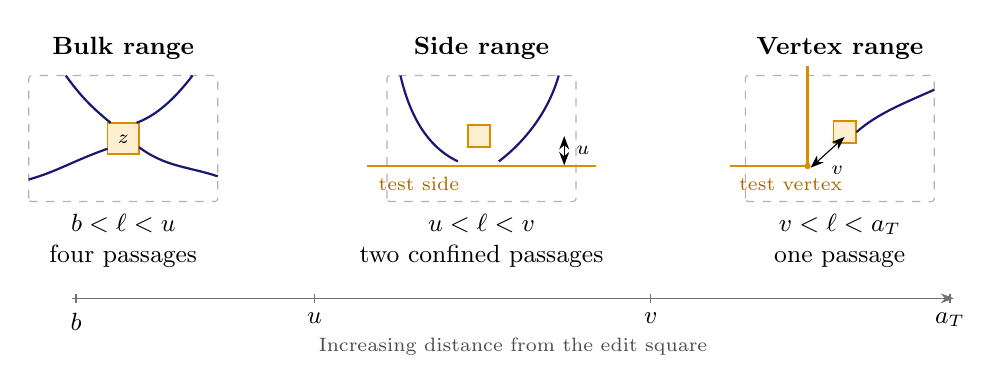
\begin{tikzpicture}[x=1cm,y=1cm,>=Stealth,
  frame/.style={draw=black!30,dashed,rounded corners=1pt},
  testedge/.style={draw=Orange!85!black,line width=1pt},
  passage/.style={draw=MidnightBlue,line width=.8pt},
  edit/.style={draw=Orange!85!black,fill=Orange!18,line width=.7pt}]
  \begin{scope}
    \node[font=\small\bfseries] at (1.75,2.2) {Bulk range};
    \draw[frame] (.55,.25) rectangle (2.95,1.85);
    \draw[edit] (1.55,.85) rectangle (1.95,1.25);
    \draw[passage] (1.55,.92) .. controls (1.12,.77) and (.91,.63) .. (.55,.53);
    \draw[passage] (1.59,1.25) .. controls (1.3,1.48) and (1.15,1.67) .. (1.02,1.85);
    \draw[passage] (1.92,1.25) .. controls (2.22,1.36) and (2.46,1.63) .. (2.63,1.85);
    \draw[passage] (1.95,.94) .. controls (2.28,.69) and (2.59,.69) .. (2.95,.57);
    \node[font=\scriptsize] at (1.75,1.04) {$z$};
    \node[font=\small,align=center] at (1.75,-.25) {$b<\ell<u$\\four passages};
  \end{scope}
  \begin{scope}[xshift=4.55cm]
    \node[font=\small\bfseries] at (1.75,2.2) {Side range};
    \draw[frame] (.55,.25) rectangle (2.95,1.85);
    \draw[testedge] (.30,.70)--(3.20,.70);
    \draw[edit] (1.58,.94) rectangle (1.86,1.22);
    \draw[passage] (1.45,.76) .. controls (1.02,.96) and (.82,1.42) .. (.72,1.85);
    \draw[passage] (1.97,.76) .. controls (2.30,1.01) and (2.60,1.39) .. (2.73,1.85);
    \draw[<->,thin] (2.80,.71)--(2.80,1.08);
    \node[font=\scriptsize,anchor=west] at (2.83,.90) {$u$};
    \node[font=\scriptsize,anchor=west,text=Orange!65!black] at (.32,.47) {test side};
    \node[font=\small,align=center] at (1.75,-.25) {$u<\ell<v$\\two confined passages};
  \end{scope}
  \begin{scope}[xshift=9.10cm]
    \node[font=\small\bfseries] at (1.75,2.2) {Vertex range};
    \draw[frame] (.55,.25) rectangle (2.95,1.85);
    \draw[testedge] (.35,.70)--(1.34,.70)--(1.34,1.97);
    \fill[Orange!85!black] (1.34,.70) circle (.04);
    \draw[edit] (1.67,.99) rectangle (1.95,1.27);
    \draw[passage] (1.96,1.13) .. controls (2.23,1.37) and (2.57,1.50) .. (2.95,1.67);
    \draw[<->,thin] (1.38,.68)--(1.81,1.07);
    \node[font=\scriptsize,anchor=north west] at (1.52,.82) {$v$};
    \node[font=\scriptsize,anchor=west,text=Orange!65!black] at (.35,.47) {test vertex};
    \node[font=\small,align=center] at (1.75,-.25) {$v<\ell<a_T$\\one passage};
  \end{scope}
  \draw[->,black!55] (1.10,-.98)--(12.30,-.98);
  \foreach \x/\lab in {1.15/b,4.18/u,8.45/v,12.25/a_T}{
    \draw[black!55] (\x,-.92)--(\x,-1.04);
    \node[below,font=\small] at (\x,-1.04) {$\lab$};
  }
  \node[font=\scriptsize,text=black!70] at (6.70,-1.59)
    {Increasing distance from the edit square};
\end{tikzpicture}

 \caption{The three geometric ranges in the pivotal-square implication.
 Orange squares indicate edits; orange sides and vertices belong to
 the test polygons, not to a pinned domain boundary.  Blue arcs represent
 the required exterior passages, schematically, at an intermediate
 scale $\ell$.  The actual checks use separated rings, may be recentered
 on a side or vertex, and omit rings near the transition scales.
 Dashed frames illustrate free neighborhoods, not literal ring placements.
 The distinction between bulk, side, and vertex locations yields the
 exponent requirements $p_4>2$, $p_h>1$, and $p_1>0$ in the location count.}
 \label{fig:pivotal-ranges}
\end{figure}
Figure~\ref{fig:pivotal-ranges} summarizes these ranges.  The scales
$u$ and $v$ locate the change from a two-dimensional set of possible
edit centers to neighborhoods of sides and then vertices.

\subsection{Local conditional laws and a single reversal}

Here and until physical lengths are explicitly introduced, distances
are in lattice units.  If $W$ is a free chart and $\zeta$ specifies the
exterior spin and reference auxiliary variables, the level-$k$
specification is
\begin{equation}
 \mu_{k,\eta,W}^{\zeta}(\dd\chi_W)
 =\frac{\exp F_{k,W}^{\zeta}(\chi_W)}
 {\mu_{{\rm pure},W}^{\zeta}(\exp F_{k,W}^{\zeta})}
 \mu_{{\rm pure},W}^{\zeta}(\dd\chi_W),
 \qquad
 F_{k,W}^{\zeta}=\sum_{i:\,\supp f_i^{(k)}\cap W\ne\varnothing}
 f_i^{(k)}(\chi_W\zeta_{W^c}).
 \label{eq:crossing-specification}
\end{equation}
The reference law is pure critical Ising times the product law of its
auxiliary variables.  At level zero, $\mu_{0,\eta,W}^{\zeta}$ is the
conditional nearest-neighbor Ising law under consideration.

We import the ``Local implementation'' and ``A coupling of consecutive
fields'' of~\cite[Section~3]{R}.  Their hypotheses are the array
hypotheses used in the scale construction: each potential is bounded,
real, spin-flip even and pure centered, with field support and primitive
environmental dependence within $Cs_k$ of its cell; the primitive
variables are independent; and the array is stationary on the scale
grid and square symmetric in law.  A finite first moment suffices for
the mark estimate below, and follows here from the fortieth moment.
No symmetry under negating a bond variable is required.

The local implementation has the following precise conditional scope.
With \emph{old} exterior field variables fixed, the step can be performed
inside $W$ and is exact.  Nontrivial fresh-coin decorations whose full
stencils leave $W$ are suppressed, their old logarithmic terms are
retained, and integrations whose full stencils leave $W$ are skipped.
All pairwise coin comparisons used to select separated parent cells
are retained, including comparisons that do not lead to an integration;
retained logarithmic terms are included in each permitted integration
they meet.  Every
nontrivially decorated fresh coin is therefore sampled inside $W$.
The output specification agrees with the full level-$(k+1)$
specification at distance at least $C_1s_{k+1}$ from $\partial W$.
Conditioning on the exterior of this eroded chart \emph{after} sampling
the output gives a mixture of its conditional specifications.  Exactness
does not assert an unchanged input kernel if the fresh coins are
independently pinned beforehand.

For fixed $\eta$, reversal changes spins only in marked squares of
radius $b_k=5s_{k+1}$ about parent centers.  The marks are independent
conditional on $\eta$ and independent of the entire output Gibbs
sample.  Choose the parameters themselves as exterior-independent
measurable functions of the local primitive-variable stencil, with
\begin{equation}
 p_{x,k}(\eta)\leq\min\left\{1,
 C_L\sum_{i:\,|s_ki-x|_\infty\leq C_Ls_{k+1}}\|f_i^{(k)}\|\right\},
 \qquad \E p_{x,k}\leq C_LX_k.
 \label{eq:crossing-marks}
\end{equation}
This applies also to the localized step and to unused candidate centers.
For example, if $S_x$ bounds the local logarithmic change, the old
conditional density is at least $e^{-S_x}$ times the new one.  Keeping
the new sample with probability $e^{-S_x}$ and otherwise sampling the
residual law proves the assertion, since $1-e^{-S_x}\leq\min\{1,S_x\}$.
Separation of the integration squares permits independent decisions.

For a check of inner radius $r$, start with
$W=S_{2ar}(z,\alpha)\setminus S_{r/2}(z,\alpha)$ and use
$W_k=W\ominus M_1s_k$, where erosion removes a layer along both
boundary components.  Choose
$M_1s_{k+1}\geq M_1s_k+C_1s_{k+1}$ and then $M_0$ large enough that
$r\geq M_0s_k$ leaves the smaller proportional collars fixed above.
Raise the first retained ring radius by a fixed factor if necessary so
all enlarged stencils fit in disjoint collars.

For marks $M$ from just one reversal and a spin sample $\sigma$, let
$\mathcal C(\sigma,M)$ be the configurations agreeing with $\sigma$
outside their marked squares.  Define
\[
 \begin{aligned}
 T^+(\sigma,M)&=\1\{T=1\text{ for some configuration in }
                         \mathcal C(\sigma,M)\},\\
 D_T(\sigma,M)&=\1\{T\text{ is nonconstant on }\mathcal C(\sigma,M)\}.
 \end{aligned}
\]
With $\pi_{k-1,\eta}$ the mark law for reversing step $k-1$, set
\begin{equation}
 B_{k,T}(\eta)=\sup_\zeta\mu_{k,\eta,W_k}^{\zeta}(T),\qquad
 B^+_{k,T}(\eta)=\sup_\zeta
       (\mu_{k,\eta,W_k}^{\zeta}\otimes\pi_{k-1,\eta})(T^+),\quad k\geq1.
 \label{eq:crossing-envelopes}
\end{equation}
Only $B_{0,T}$ is used at level zero.  Each supremum is a finite maximum:
only finitely many exterior variables can enter the chart, and their
alphabets are finite.  It is consequently measurable and depends only
on primitive environmental variables in the chart and a fixed
$O(s_k)$ neighborhood.  Taking the supremum \emph{before} environmental
expectation preserves this locality and bounds arbitrary mixtures of
exterior assignments: each fixed exterior kernel uses the same local
primitive variables, so maximizing over exterior values introduces no
additional environmental variables.

\begin{lemma}[Error from one reversal]
\label{lem:crossing-one-step}
Consider a fixed buffered test $T$ under a level-$k$ specification, with
marks from step $k-1$.  Suppose every retained ring check satisfies
$\E B^+_{k,T_i}\leq q_i^0+\tau_i$.  Retain rings only beyond a fixed
large multiple of $s_k$, with their collars enlarged by all field,
mark, and environmental stencils disjoint and avoiding the inserted
mark's primitive-variable stencil.  There is $c>0$, independent
of $T$, such that
\begin{equation}
 \E\sup_\zeta(\mu_{k,\eta}^{\zeta}\otimes\pi_{k-1,\eta})(D_T)
 \leq C_TX_{k-1}\min\{1,(s_k/a_T)^c\}.
 \label{eq:crossing-one-step}
\end{equation}
The same estimate bounds $T^+-T$, and holds for deterministic partial
activation of the marks.  Constants are uniform over the placements
and dilations of the three fixed check shapes.
\end{lemma}

\begin{proof}
Hold the output spin sample fixed and activate relevant squares in a
deterministic order.  The first square
whose addition permits two values of $T$ is pivotal for some assignment
inside the preceding squares.  Reverting only the new square in that
assignment shows that the passages forced by
\eqref{eq:crossing-pivotal-distances} are possible using previous marks.
Enlarging to all other marks in each ring can only increase this event.

For an inserted mark at $x$ and retained rings $T_1,\ldots,T_m$, condition
on all Gibbs variables outside one eroded ring chart and on all marks
whose squares do not meet its test support.  The enlarged collars put
every square relevant to this support inside the chart and make the
other ring events measurable under this conditioning.  The remaining
field has conditional law~\eqref{eq:crossing-specification}, with every potential
touching the chart included, and the remaining marks retain their
independent law.  This conditions on output auxiliary variables only
after their joint law has been constructed.  It does not condition on
the reconstructed old spins or on the other possibility events themselves.
Iterating gives
\begin{equation}
 \sup_\zeta\bigl[p_{x,k-1}(\eta)
       \Prob_{k,\eta}^{\zeta}(T_1^+\cap\cdots\cap T_m^+)\bigr]
 \leq p_{x,k-1}(\eta)\prod_{\ell=1}^m B^+_{k,T_\ell}(\eta).
 \label{eq:crossing-conditional-product}
\end{equation}
The ring neighborhoods are disjoint and avoid the primitive-variable
stencil of $p_{x,k-1}$.  Independence of these primitive variables,
including the priorities and thresholds, therefore gives
\begin{equation}
 \E\left[p_{x,k-1}\prod_{\ell=1}^m B^+_{k,T_\ell}\right]
 =\E p_{x,k-1}\prod_{\ell=1}^m\E B^+_{k,T_\ell}
 \leq C_LX_{k-1}\prod_{\ell=1}^m(q_{i(\ell)}^0+\tau_{i(\ell)}).
 \label{eq:crossing-independent-product}
\end{equation}
This factorization uses no property of the one-edge distribution beyond
primitive independence.  Unconditional quenched passage probabilities
would not provide the local factors needed for it.

Let $b=5s_k<a_T$.  Rings of ratio $a$ spaced in ratio $Ga$ and
\eqref{eq:crossing-slack} bound the last product, including the bounded
losses at transitions, by
\[
 C_T(b/u)^{p_4}(u/v)^{p_h}(v/a_T)^{p_1}.
\]
Normalize $a_T=1$.  Centers in a dyadic distance class $(u,v)$ occupy
area at most $C_Tuv$: near a vertex the relevant side length is $O_T(v)$
and its transverse width is $O(u)$; the class $u=v=1$ includes the
remaining interior.  Since centers have spacing comparable to $b$,
there are at most $C_Tuv/b^2$ such centers, including cell overhangs.
Their total contribution is at most
\[
 C_TX_{k-1}(b/u)^{p_4-2}(u/v)^{p_h-1}v^{p_1}.
\]
The three ratios multiply to $b$, so this is bounded by
$C_TX_{k-1}b^d$ for $d=\min\{p_4-2,p_h-1,p_1\}>0$.
There are $O_T((1+\log(1/b))^2)$ classes; absorbing this factor gives
$c=d/2$.  If $b\geq a_T$, only a bounded number of candidate squares
meet the fixed test, and the crude mark estimate suffices.  Finally,
$T^+-T\leq D_T$, and partial activation decreases the possibility events.
\end{proof}

\subsection{Closing the fixed-shape bootstrap}

\begin{lemma}[Uniform conditional passage bounds]
\label{lem:crossing-bootstrap}
There is a fixed $x_{\rm cr}>0$ such that $\sup_jX_j\leq x_{\rm cr}$
implies, for each of the three checks $T_i$ with inner radius
$r\geq M_0s_k$,
\begin{align}
 \E B_{k,T_i}
 &\leq q_i^0+C_{\rm b}\sum_{j=k}^{J(r)}X_j(s_j/r)^c,
 \label{eq:crossing-bootstrap-plain}\\
 \E B^+_{k,T_i}
 &\leq q_i^0+C_{\rm b}\sum_{j=k}^{J(r)}X_j(s_j/r)^c
               +C_{\rm b}X_{k-1}(s_k/r)^c,\qquad k\geq1,
 \label{eq:crossing-bootstrap-possible}
\end{align}
where $J(r)=\max\{j:M_0s_j\leq r\}$.  Both upper bounds are at most
$q_i^0+\tau_i$.  They hold for all placements, including embedded bulk
torus charts, with arbitrary exterior Gibbs data.
\end{lemma}

\begin{proof}
Use strong induction on dyadic ranges of $r/s_k$, simultaneously for
all levels and placements.  At terminal ratios
$M_0s_k\leq r<M_0s_{k+1}$ only a bounded number of potentials meet the
chart.  If $S$ is their total norm, the bounded logarithmic tilt in
\eqref{eq:crossing-specification} gives
\[
 \sup_\zeta\|\mu_{k,\eta,W_k}^{\zeta}
                  -\mu_{{\rm pure},W_k}^{\zeta}\|_{\TV}
 \leq\min\{1,2S\},\qquad \E S\leq C X_k.
\]
Since $(s_k/r)^c\geq(M_0L)^{-c}$, this proves the terminal plain bound
with a fixed $C_{\rm b}$.

For a nonterminal plain check, the local scale change expresses the new
interior law as a mixture of level-$(k+1)$ specifications.  Its plain
check has smaller ratio $r/s_{k+1}$.  Every ring controlling the reversal
has inner radius at most $r/2$, is evaluated at level $k+1$, and has
the required free collars.  Its ratio to its spacing lies in a strictly
smaller induction range.  The inductive possibility estimates therefore
justify Lemma~\ref{lem:crossing-one-step}, at cost
$CX_k(s_{k+1}/r)^c$.  This is a fixed multiple of the $j=k$ term in
\eqref{eq:crossing-bootstrap-plain}; the next-level plain bound supplies
the remaining terms.

After proving the plain bound at a given ratio, compare its possibility
event using marks from step $k-1$.  Its rings are now evaluated at level
$k$, still have inner radii at most $r/2$, and hence again belong to
strictly smaller induction ranges.  Lemma~\ref{lem:crossing-one-step}
adds $CX_{k-1}(s_k/r)^c$.  If no admissible ring fits, the test and edit
scales differ by a bounded factor, so a bounded count of candidate marks
gives the same estimate.  This also starts the terminal possibility
induction without a circular appeal to a passage estimate at its own
ratio.

The errors remain within the fixed tolerances because
\begin{equation}
 \sum_{j=k}^{J(r)}(s_j/r)^c
 \leq\frac{M_0^{-c}}{1-L^{-c}}.
 \label{eq:crossing-geometric-sum}
\end{equation}
Choose $C_{\rm b}$ to cover the terminal and one-step constants, and
then choose $x_{\rm cr}$ so that $C_{\rm b}x_{\rm cr}$ times this bound,
plus the additional single-level term, is below $\min_i\tau_i$.
These choices use only the three fixed check shapes and the fixed scale
parameters.  Each invocation of the induction uses precisely these
tolerances, which closes both estimates.
\end{proof}

Lemma~\ref{lem:crossing-one-step} now applies to every prescribed finite
family of buffered polygonal tests.  Such a family changes its constants
$C_T,a_T$, but does not change $x_{\rm cr}$.  The remaining convergence
arguments use the elementary consequence of geometric spacing
\begin{equation}
 \sum_{j<K}X_j\min\{1,(s_{j+1}/r)^c\}+X_K\longrightarrow0
 \label{eq:crossing-weighted-decay}
\end{equation}
as $r,K\to\infty$, provided $s_K/r$ stays between fixed positive bounds.
Indeed the sum of the weights is uniformly bounded.  For $j\geq m$
bound $X_j$ by $\sup_{j\geq m}X_j$, and for the finitely many $j<m$
let $r\to\infty$.  Then let $m\to\infty$.  This is where decay, rather
than summability, is sufficient.

\subsection{The three geometric consequences}

\begin{proposition}[Uniform local conditional comparison]
\label{prop:local-comparison}
Assume the array hypotheses above and~\eqref{eq:crossing-hypothesis}.
Fix a bounded polygonal window with a finite family $\mathcal T$ of
corridor crossings, band circuits, or passage checks, strictly inside
specified free buffers.  Annular windows may have an inner and an outer
free collar.  Dilate the whole geometry by $r\to\infty$ in lattice units.
There is an exterior-independent measurable envelope $\mathcal E_r(\eta)$
with $\E\mathcal E_r\to0$, uniformly over translations and scale-grid
positions, such that every level-zero conditional test-vector law is
within $\mathcal E_r(\eta)$ in total variation of a mixture of pure
conditional test-vector laws on a still-buffered interior window.

Consequently, if an event in the test vector has pure conditional
probability at least $c_*>0$ under all exterior assignments after a
sufficiently small fixed erosion of the buffers, its level-zero
probability is at least any $c<c_*$, uniformly over exterior assignments,
outside an environmental event of probability tending to zero.  For a
nearest-neighbor initial law, the event that this worst-boundary lower
bound holds depends only on the bonds in the window and its incident
layer.
\end{proposition}

\begin{proof}
Choose a terminal level with $s_K/r$ between two sufficiently small
fixed positive constants.  The cumulative erosion has width $O(s_K)$,
so all tests retain their prescribed buffers.  At each reversal,
\eqref{eq:crossing-conditional-product} supplies an error bound for
every exterior assignment before taking any mixture.  Concretely it is
the sum over inserted centers of their mark parameters times the
products of the appropriate ring envelopes, or just the mark parameters
when no ring fits.  Summing over the finite family and steps gives an
envelope whose expectation is bounded by
\begin{equation}
 \E\mathcal E_r\leq C_{\mathcal T}
 \left(\sum_{j<K}X_j\min\{1,(s_{j+1}/r)^c\}+X_K\right).
 \label{eq:crossing-local-error}
\end{equation}
The final term comes from deleting the bounded number of level-$K$
potentials touching the remaining window, using the logarithmic-tilt
bound in the preceding proof.  Conditional on the final exterior this
leaves the pure law, and disintegration gives the stated mixture.
Equation~\eqref{eq:crossing-weighted-decay} proves convergence.

Every member of the pure mixture gives the selected event probability
at least $c_*$.  Thus every initial exterior assignment gives probability
at least $c_*-\mathcal E_r$.  Average this inequality over the algorithmic
choices conditional on the original bond environment $\omega$, then
apply Markov's inequality.  The resulting exceptional probability is
at most $\E\mathcal E_r/(c_*-c)$.  Although the bounding envelope may use
more variables, the actual worst-boundary probability in the initial
nearest-neighbor law uses only the window bonds and incident layer;
its lower-bound event is therefore local.  Uniformity means a bound for
each placement with the same error rate, not simultaneous success at
all placements.
\end{proof}

\begin{proposition}[Expected total variation for torus tests]
\label{prop:torus-tests}
Assume the same array hypotheses and~\eqref{eq:crossing-hypothesis}.
Fix finitely many buffered tests $\mathcal T$ in a common planar chart,
now in physical units.  Let $\delta\downarrow0$ and choose tori of lattice
period $Ms_K$, with $M$ a sufficiently large fixed integer, $K\to\infty$,
and physical periods $\delta Ms_K$ in a fixed compact subinterval of
$(0,\infty)$ large enough for the chart and the complete scale stencils
to embed.  Give the torus iid bonds with the original law.  If
$\nu_{\omega}^{\mathcal T}$ and $\nu_{\rm pure}^{\mathcal T}$ are the
initial quenched and pure critical laws of the whole Boolean test vector,
then
\begin{equation}
 \E_{\omega}\|\nu_{\omega}^{\mathcal T}
                     -\nu_{\rm pure}^{\mathcal T}\|_{\TV}\longrightarrow0.
 \label{eq:crossing-torus-tv}
\end{equation}
Such tori can be chosen for every deterministic mesh sequence.
\end{proposition}

\begin{proof}
Embedded stencils have exactly their plane primitive-variable laws and
the disjointness properties used above.  Couple consecutive levels at
fixed enlarged environment.  The expected error for test $T$ at step
$j$ is at most
\[
 C_TX_j\min\{1,(\delta s_{j+1}/a_T^{\rm phys})^c\},
\]
by Lemmas~\ref{lem:crossing-one-step} and~\ref{lem:crossing-bootstrap}.
Their sum tends to zero by the same geometric-weight argument as
\eqref{eq:crossing-weighted-decay}.  At level $K$ the torus contains
$O(M^2)$ potentials, whose expected total norm is $O_M(X_K)$.
Deleting them couples the entire terminal law to the pure torus with
vanishing expected total variation.  Glue these couplings and take a
union bound over steps and the fixed test list.  No estimate on the union
of marks from different levels is needed.

The initial test law depends only on $\omega$, whereas the final pure
law is deterministic.  Averaging the coupling bounds over algorithmic
choices therefore proves exactly~\eqref{eq:crossing-torus-tv}, rather
than merely comparison of annealed test laws.  Finally, choosing $K$ as
the first scale with $s_K\geq A\delta^{-1}$, for a sufficiently large
fixed $A$, places the physical periods between $MA$ and $MAL$.
\end{proof}

\begin{corollary}[No interior four-passage bottlenecks]
\label{cor:four-passages}
At $\beta_*$, let $F$ be a fixed compact set with positive clearance
inside the free part of the approximating domains, and choose a
sufficiently small fixed physical radius $R>0$ so that the required
annular charts about $F$ remain free.  Uniformly over all exterior spin
assignments,
\begin{equation}
 \lim_{r\downarrow0}\limsup_{\delta\downarrow0}
 \E_{\omega}\mu_{\omega}\bigl(
 \text{four contour passages from }r\text{ to }R
                       \text{ about some }z\in F\bigr)=0.
 \label{eq:crossing-four-passages}
\end{equation}
Passages have the parameter-interval multiplicities specified above.
Fixed-factor changes of radii and local contour redrawing errors are
permitted after corresponding crops.
\end{corollary}

\begin{proof}
At a fixed center, pack rings of ratio $a$, separated by factor $G$,
between a fixed multiple of $r$ and a fixed fraction of $R$.  For fixed
physical $r>0$, their lattice radii exceed $M_0s_0$ once the mesh is
small.  Conditioning off their charts as in
\eqref{eq:crossing-conditional-product}, and then applying
\eqref{eq:crossing-independent-product} without an inserted mark,
bounds the passage probability by the product of the plain envelopes.
Their expectations are at most $q_4^0+\tau_4<(Ga)^{-p_4}$.
Consequently the mesh upper limit is at most $C(r/R)^{p_4}$, uniformly
over the ambient exterior data.

Cover $F$ by an $r$-grid with $O_F(r^{-2})$ centers.  Enlarging the inner
radius and decreasing the outer radius by fixed factors makes four
passages about any point imply a grid check.  The union bound gives
$C_{F,R}r^{p_4-2}$ after the mesh limit.  Since $p_4>2$, this tends to
zero.  The same crops absorb lattice rounding and the local matched
drawings of the resolved contours.
\end{proof}

The initializations and their scale outputs satisfy every array
hypothesis used here.  Proposition~\ref{prop:two-trajectories} makes
the uniform bound on $X_k$ in~\eqref{eq:crossing-hypothesis} as small as needed
by reducing $\varepsilon_0(\rho)$, and makes $X_k$ decay.  The fixed
threshold $x_{\rm cr}$ depends only on the three check shapes and the
scale parameters.  Thus this reduction of $\varepsilon_0(\rho)$ precedes
the choice of a final domain, test family, or approximation sequence.
Proposition~\ref{prop:matching} places these conclusions on both lattices
at $\beta_*$.  The local comparison will give FK annular barriers; the
torus comparison and four-passage exclusion will control the interface.

\section{Identification of the physical critical point}
\label{sec:criticality}

The matched temperature $\beta_*$ was selected by the scale map. To
identify it with the magnetization threshold, we first construct local
FK barriers at $\beta_*$ on both lattices. These barriers rule out
percolation at the matched temperature. Above $\beta_*$, the dual odds
decrease; a decision-tree argument then makes dual connections rare
enough to force primal percolation. This is the local sharpness
argument of~\cite[Section~8]{R}, applied to the exact dual family
rather than to a distributionally self-dual model.

Write $B_r(x)=\{y:|y-x|_\infty\le r\}$ on the lattice under
consideration; radii may be rounded to integers. Let
$\phi_{\beta,\omega}^{\mathrm w}$ be the primal infinite-volume
wired FK measure. It is obtained by decreasing limits of finite
wired-box laws on local increasing events, and the limit does not
depend on the exhaustion. The analogous notation with a star refers
to the dual odds at the same physical parameter $\beta$.

\subsection{Annular barriers at the matched temperature}

\begin{lemma}[Local FK barriers on both lattices]
\label{lem:fk-barriers}
There exist $a_0>1$ and $c_0>0$ with the following property, separately
for the primal and dual lattices. Let $\mathcal A(x,r)$ be the annular
graph between the lattice layers of radii $r$ and $a_0r$, and let
$\mathcal R(x,r)$ be the event of an ordinary open path between
these layers. Call its bond environment good if
\begin{equation}
 \phi_{\mathcal A(x,r),\beta_*,\omega}^{\mathrm w}
        (\mathcal R(x,r))\le1-c_0,
 \label{eq:good-annulus}
\end{equation}
using the odds of that lattice and wiring both boundary components
together. Goodness depends only on the original bonds in the annulus
and an incident layer, and
\begin{equation}
 \sup_x\Prob\bigl(\mathcal A(x,r)\text{ is not good}\bigr)
                         \longrightarrow0\qquad(r\to\infty).
 \label{eq:annulus-good-probability}
\end{equation}
For a good annulus, the same crossing upper bound holds with any
less wired boundary condition and after any decrease in its edge odds.
In particular,
\begin{equation}
       \E_\rho\phi_{\beta_*,\omega}^{\mathrm w}
                      (0\leftrightarrow\infty)=0.
 \label{eq:no-percolation-at-matching}
\end{equation}
\end{lemma}

\begin{proof}
Choose $a_0$ large enough to place two disjoint annular subbands
between the boundary layers, with positive-width free buffers around
each. In the pure critical Ising model, simultaneous plus and minus
spin circuits, one in each subband, have probability at least
$2c_0>0$, uniformly over spin pins beyond those buffers. This is
\cite[Section~2, Proposition ``Pure buffered RSW consequences'']{S}:
the two prescribed colors have disjoint buffered rectangle
constructions. Fix the subbands with enough clearance that a small
erosion of the buffers preserves this lower bound.

Proposition~\ref{prop:local-comparison}, applied to these two circuit
tests, transfers the lower bound to the quenched model, with
environmental probability tending to one. Proposition~\ref{prop:matching}
makes this comparison available for both the primal and dual arrays
at $\beta_*$. Apply it to Edwards--Sokal spins for the annular FK
measure with its fully wired boundary cluster pinned plus. Every
ordinary open FK path has constant spin. A radial path would have
to meet both separating circuits, and hence could not be open.
The triangulation used for the spin tests causes no exception:
ordinary nearest-neighbor edges cannot cross a triangulated circuit
without meeting one of its vertices. Thus the simultaneous circuit
event implies the complement of $\mathcal R(x,r)$ and proves
\eqref{eq:good-annulus} outside an event of probability tending to
zero.

Defining goodness by the original finite-volume FK probability in
\eqref{eq:good-annulus} removes the auxiliary random choices of the
scale construction. It is a measurable function of the stated local
bond set. The all-exterior-pin scope of
Proposition~\ref{prop:local-comparison} gives
\eqref{eq:annulus-good-probability} uniformly in placement.
Monotonicity in the odds and in boundary wiring gives the remaining
finite-volume assertion.

To deduce \eqref{eq:no-percolation-at-matching}, choose concentric
annuli with a fixed large geometric separation, so that their full
bond neighborhoods are disjoint. Start at a radius beyond which
the probability of a bad annulus is at most $1/2$. For annulus $i$
put $a_i(\omega)=1-c_0\1_{\{i\text{ is good}\}}$. In any containing
finite wired box $G$, condition on all edges off this annulus. Its
conditional law has a boundary partition dominated by full wiring;
therefore
\[
 \phi_{G,\beta_*,\omega}^{\mathrm w}
       (\mathcal R_i\mid\text{edges off annulus }i)
                \le a_i(\omega).
\]
Successively applying these conditional bounds shows that the
probability of crossing $\ell$ such annuli is at most
$\prod_{i=1}^{\ell}a_i(\omega)$. No independence of FK crossings
is asserted here. Independence of the original bond neighborhoods
does give
\[
 \E_\rho\prod_{i=1}^{\ell}a_i(\omega)
       =\prod_{i=1}^{\ell}\E_\rho a_i(\omega)
       \le(1-c_0/2)^\ell.
\]
The same local bounds pass to the wired infinite-volume limit.
Every infinite path crosses all the annuli, so letting
$\ell\to\infty$ proves the claim.
\end{proof}

\subsection{Dual arms above the matched temperature}

The local comparison supplies no rate in
\eqref{eq:annulus-good-probability}. We first obtain a useful rate
by using disjoint bond sets in many separated annuli at each center.
The resulting environmental exceptional probability decays faster
than every power of the box size. Outside this exceptional set a
layer exploration has small revealment, and the weighted derivative
strengthens polynomial arm decay to a stretched exponential bound.

\begin{lemma}[Rapid annealed decay of dual arms]
\label{lem:dual-arms}
For every $\beta'>\beta_*$ and $A>0$ there is a finite constant
$C_{\beta',A}$ such that, on the dual lattice,
\begin{equation}
 \E_\rho\phi_{B_{2N}(x),\beta',\omega}^{\mathrm w,*}
  \bigl(x\leftrightarrow\partial B_N(x)
                    \text{ inside }B_N(x)\bigr)
                     \le C_{\beta',A}N^{-A}.
 \label{eq:dual-arm-bound}
\end{equation}
The estimate is uniform in the center. It also holds for the same
ordinary path event under any finite or infinite-volume dual FK law
whose domain contains $B_{2N}(x)$, with arbitrary boundary conditions
outside that box.
\end{lemma}

\begin{proof}
Fix $x$. For every $z\in B_{N+1}(x)$, choose
$\ell_N\asymp\log N$ concentric annuli of the type in
Lemma~\ref{lem:fk-barriers}, with inner radii between $N^{1/4}$
and a sufficiently small multiple of $N^{1/2}$. Choose their
geometric spacing so that their full bond neighborhoods are disjoint
and all lie inside $B_{N^{1/2}}(z)$. Let $\eta_N$ be an upper bound
for their bad-environment probabilities, uniformly over centers and
the selected radii. Equation~\eqref{eq:annulus-good-probability}
gives $\eta_N\to0$.

Independence of the annuli at one fixed center shows that
\[
 \Prob\bigl(\text{at least }\ell_N/2
                       \text{ annuli at }z\text{ are bad}\bigr)
                  \le2^{\ell_N}\eta_N^{\ell_N/2}.
\]
Let $\mathcal G_N$ be the event that fewer than half the annuli
are bad at every $z\in B_{N+1}(x)$. A union bound gives
\begin{equation}
 \Prob(\mathcal G_N^c)
       \le C N^2 2^{\ell_N}\eta_N^{\ell_N/2}
       =o(N^{-A})\qquad\text{for every }A>0.
 \label{eq:amplified-environment-bound}
\end{equation}
Indeed, $\ell_N$ is bounded above and below by positive multiples
of $\log N$, while $\log(1/\eta_N)\to\infty$. There is no
independence assertion between the annulus families at different
centers.

In an environment in $\mathcal G_N$, multiply the conditional
annulus bounds exactly as in the preceding proof. Since the dual
odds decrease as $\beta$ increases, the same environment gives
\begin{equation}
 \phi_{B_{2N}(x),\beta,\omega}^{\mathrm w,*}
 \bigl(z\leftrightarrow\partial B_{N^{1/2}}(z)
                 \text{ inside }B_{N^{1/2}}(z)\bigr)
       \le(1-c_0)^{\ell_N/2}
       \le C N^{-\alpha}
 \label{eq:uniform-short-dual-arms}
\end{equation}
for a fixed $\alpha>0$, all $z\in B_{N+1}(x)$, and every
$\beta\in[\beta_*,\beta']$. For large $N$ all the small boxes
are contained in $B_{2N}(x)$; their induced boundary conditions are
covered by full annular wiring.

Fix such an environment and let
\[
 q_\omega(\beta)=\phi_{B_{2N}(x),\beta,\omega}^{\mathrm w,*}
  \bigl(x\leftrightarrow\partial B_N(x)
                    \text{ inside }B_N(x)\bigr).
\]
Choose an integer $i$ uniformly between $N/4$ and $N/2$, and explore
all ordinary open clusters in $B_N(x)$ that meet the layer
$\partial B_i(x)$. This exploration determines the event defining
$q_\omega$: any path from $x$ to $\partial B_N(x)$ meets the
chosen layer, and all clusters meeting it have been completely
explored inside $B_N(x)$. This adapts the layer exploration in
\cite[Lemma~3.2 and its proof]{DCRT}.

An edge is queried only when an endpoint lies on, or has an ordinary
open path to, the chosen layer. For each fixed endpoint $z$, the
fraction of choices of $i$ whose layer comes within distance
$2N^{1/2}$ of $z$ is at most $C N^{-1/2}$. For any other choice,
the connection to the layer forces an ordinary arm from $z$ to
$\partial B_{N^{1/2}}(z)$. Thus
\eqref{eq:uniform-short-dual-arms} gives
\begin{equation}
 \max_e\delta_e
       \le C\bigl(N^{-1/2}+N^{-\alpha}\bigr)
       \le C N^{-d},\qquad d=\min\{1/2,\alpha\}>0.
 \label{eq:layer-revealment}
\end{equation}
The tree queries only edges in $B_N(x)$, but its law is the full
wired measure on $B_{2N}(x)$. In particular, it never follows a
wired boundary identification. Edges outside $B_N(x)$ have zero
revealment.

All finite odds are positive, so $0<q_\omega(\beta)<1$.
Apply \eqref{eq:fk-osss} to this finite wired measure. In the
dual version of \eqref{eq:weighted-derivative}, the coefficients
of $-q_\omega'$ are $a_e(\beta)$, uniformly bounded below on
$[\beta_*,\beta']$. Covariances for edges outside the explored
box remain nonnegative. Consequently
\begin{equation}
 -q_\omega'(\beta)
       \ge c_{\beta'} N^d q_\omega(\beta)(1-q_\omega(\beta)),
       \qquad \beta\in[\beta_*,\beta'].
 \label{eq:dual-differential-inequality}
\end{equation}
Moreover \eqref{eq:uniform-short-dual-arms} at $z=x$ gives
$q_\omega(\beta_*)\le C N^{-\alpha}$. Integrating the derivative
of the logit, for all sufficiently large $N$,
\[
 \frac{q_\omega(\beta')}{1-q_\omega(\beta')}
 \le\frac{q_\omega(\beta_*)}{1-q_\omega(\beta_*)}
       e^{-c_{\beta'}(\beta'-\beta_*)N^d}
 \le e^{-c_{\beta'}(\beta'-\beta_*)N^d}.
\]
Averaging this estimate on $\mathcal G_N$ and using
\eqref{eq:amplified-environment-bound} on its complement proves
\eqref{eq:dual-arm-bound}. In a larger graph, condition outside
$B_{2N}(x)$ and dominate the induced boundary partition by full
wiring. This proves the final assertion, which then passes to
infinite-volume limits.
\end{proof}

\subsection{Percolation and plus magnetization}

\begin{proposition}[Physical criticality]
\label{prop:physical-criticality}
For the original iid bond law and every sufficiently small fixed
$\varepsilon>0$, the temperature in
Proposition~\ref{prop:matching} satisfies
\begin{equation}
                    \beta_* = \beta_c^\rho(\varepsilon).
 \label{eq:physical-critical-point}
\end{equation}
The environmental mean of the infinite-volume plus magnetization
is zero for $0\le\beta\le\beta_*$ and strictly positive for every
$\beta>\beta_*$.
\end{proposition}

\begin{proof}
By Lemma~\ref{lem:fk-barriers} and monotonicity,
\[
 \E_\rho\phi_{\beta,\omega}^{\mathrm w}
          (0\leftrightarrow\infty)=0,
                    \qquad0<\beta\le\beta_*.
\]
Fix $\beta'>\beta_*$. Finite planar FK duality sends the primal
odds to $2/w_e(\beta')$, exactly the dual family considered in
Lemma~\ref{lem:dual-arms}. In each buffered interior box the
induced dual boundary condition is dominated by full wiring. Thus
the lemma bounds ordinary closed-dual arms under finite primal
wired laws and, by taking local limits, under
$\phi_{\beta',\omega}^{\mathrm w}$. Only this local comparison
is needed; no distributional self-duality is used.

A closed-dual circuit surrounding $B_m(0)$ whose maximal distance
from the origin lies in $[R,2R)$ has diameter at least $cR$.
It therefore contains an ordinary dual arm reaching distance $c'R$
from some dual vertex in $B_{2R+1}(0)$. Sum
\eqref{eq:dual-arm-bound} over the $O(R^2)$ possible vertices,
using the bound with its surrounding collar, and then over dyadic
$R$ comparable with or larger than $m$. For any $A>2$ this gives
\begin{equation}
 \E_\rho\phi_{\beta',\omega}^{\mathrm w}
   \bigl(\text{a closed-dual circuit surrounds }B_m(0)\bigr)
       \le C_{\beta',A}\sum_{j\ge0}(2^j m)^{2-A}
                           \longrightarrow0.
 \label{eq:surrounding-dual-circuits}
\end{equation}

If every open cluster meeting $B_m(0)$ were finite, their finite
union would contain the box and would be connected as a vertex
set: each of its vertices is joined by an open path to the box,
and the box itself is nearest-neighbor connected. Every outgoing
edge of this union is closed. Its outer dual boundary therefore
contains a surrounding closed-dual circuit: one may first fill the
finite complementary components, after which all edges toward the
infinite complementary component are still closed. The complement of the
event in \eqref{eq:surrounding-dual-circuits} forces an infinite
open cluster to meet $B_m(0)$. For all sufficiently large $m$ this
has positive probability under the joint environment--FK law.
That law is translation invariant: the environment is iid and
the wired infinite-volume specification is covariant under
translations. Hence
\[
 0<\E_\rho\phi_{\beta',\omega}^{\mathrm w}
             (B_m(0)\leftrightarrow\infty)
 \le |B_m(0)|\,
       \E_\rho\phi_{\beta',\omega}^{\mathrm w}
             (0\leftrightarrow\infty).
\]
This proves positive expected wired percolation for every
$\beta'>\beta_*$.

It remains to identify this order parameter with the precise plus
magnetization used in the definition of $\beta_c^\rho(\varepsilon)$.
Fix an environment and $\beta>0$. In the finite spin box, include
all bonds with at least one endpoint in that box and wire the exterior
endpoints, pinning their cluster plus. Edwards--Sokal gives
\[
 \langle\sigma_0\rangle^+_{B_m,\beta,J}
       =\phi^{+,m}_{\beta,\omega}
               (0\leftrightarrow\text{wired exterior boundary}).
\]
For these square boxes the boundary probability is exactly
$u_{m+1}(\omega)$, where $u_n$ is the root-to-boundary probability
in the ordinary wired box $B_n$. Indeed, completing the exterior
endpoints to $\partial B_{m+1}$ adds only wired vertices and
wired-to-wired edges, which do not affect this probability.
The monotone limit of $u_n$ exists. To identify it with percolation
in the local infinite-volume limit, first use wired domination:
\[
 \phi_{\beta,\omega}^{\mathrm w}(0\leftrightarrow\infty)
                         \le u_m(\omega)
 \quad\text{for every }m.
\]
Conversely, for every fixed $r<m$, the root-to-boundary event in
$B_m$ implies an ordinary connection from $0$ to $\partial B_r$.
Taking $m\to\infty$ for this local event and then $r\to\infty$
shows
\[
 \lim_m u_m(\omega)
       \le\lim_r\phi_{\beta,\omega}^{\mathrm w}
                    (0\leftrightarrow\partial B_r)
       =\phi_{\beta,\omega}^{\mathrm w}(0\leftrightarrow\infty).
\]
The equality with $u_{m+1}$ gives the same limit for the exterior-plus
convention. Thus, in each environment,
\begin{equation}
 \lim_{m\to\infty}\langle\sigma_0\rangle^+_{B_m,\beta,J}
       =\phi_{\beta,\omega}^{\mathrm w}(0\leftrightarrow\infty).
 \label{eq:magnetization-percolation}
\end{equation}
All variables lie in $[0,1]$, so environmental expectations preserve
this equality. At $\beta=0$ the magnetization is zero directly.
The vanishing and positivity already proved establish
\eqref{eq:physical-critical-point} from the definition of the
critical inverse temperature.
\end{proof}

\section{Signed barriers and the quenched interface limit}
\label{sec:interface}

By Proposition~\ref{prop:physical-criticality}, the common tuning parameter is
$\beta_* =\beta_c^\rho(\varepsilon)$.  We now use the finite-vector
comparison of Proposition~\ref{prop:torus-tests} to place the target
interface between two pure comparison interfaces.  The comparisons
will preserve the pure marginal conditional on the original bond
environment.  This is the property that will yield convergence of
quenched laws, rather than only convergence after averaging over bonds.
Throughout this section, probabilities without an environmental
subscript include spins and coupling randomness as well as bonds.

\subsection{Boundary conventions and signed geometry}

Fix a bounded Jordan domain $D$, distinct marks $a,b\in\partial D$,
and the deterministic approximations in Theorem~\ref{thm:main}.
Write $D_n$ for their domains in physical coordinates, after
multiplication by $\delta_n$.  A lattice Jordan domain here is a full
square-lattice domain: bonds have not been deleted in its interior.
One standard convention surrounds the union of closed square cells
centered at the free spin sites, fixes the exterior nearest neighbors,
and retains every bond incident to a free spin.  The interface then
has a local half-edge at each boundary change.  Equivalently one can
use a lattice polygon made of plaquettes, with the boundary vertices
pinned and all interior vertices free.  The argument below applies to
both conventions.  In the first convention the exterior pin assignment
is an actual assignment to sites, so repeated incidences at one site
must have the same value.  The marked boundary changes and any
half-edge endpoints differ by at most $O(\delta_n)$.

We may take the boundary homeomorphisms to match the marks exactly.
Indeed, their inverse images of the discrete marks converge to $a,b$;
in a fixed circle parametrization, precompose by circle homeomorphisms
converging uniformly to the identity and taking $a,b$ to those inverse
images.  After passage to a subsequence the designation of the plus
arc is fixed.  Denote the open limiting arcs by $I_+$ and $I_-$.
Thus boundary order and signs, as well as positions, converge.
Winding number stability then implies that each compact subset of $D$
is eventually inside $D_n$, and each compact subset of
$\C\setminus\overline D$ is eventually outside $D_n$.

Let $\Gamma_n$ be the target contour, oriented from the mark near $a$
to the mark near $b$.  Its conditional law given the original
environment $\omega$ is $Q_{n,\omega}$.  We use the prescribed NE/SW
resolution, or a simple drawing of the same resolution inside small
vertex disks.  Matching the contour pieces in their traversal order
changes $d_{\rm curv}$ by $O(\delta_n)$.  The resolved graph has degree
two except at its two marked ends, so this drawing of its connecting
component is a simple arc.  Spin paths use the fixed triangulation by
NW/SE diagonals from the crossing section.  In the bulk its zero
contours have precisely these resolved connections.

We next describe the boundary placements used in
\cite[Section~9, ``Displaced domains and finite boundary barriers'']{R}
and \cite[Section~7, ``Fixed displaced domains and their boundary
incidences'']{S}.  To obtain the lower pure comparison, move the middle
plus boundary outward and the minus boundary inward.  Two cuts allow
comparison through a torus: a plus crossing screens the comparison
domain's plus boundary, and a minus crossing screens the target's minus
boundary.  After revealing these crossings, the remaining boundary
incidences have the orders needed for two comparisons with identical
couplings.  The strips on the central side of both cuts will transfer
signed barriers between the domains.

Fix a plane Schoenflies homeomorphism $\Psi$ taking
the unit disk to $D$, $1,-1$ to $a,b$, and the upper semicircle to
$I_+$.  These coordinates describe topology only; all tests below are
polygonal tests in the physical plane.

For small $h>0$, first take a radial boundary equal to $1+3h$ on
$[4h,\pi-4h]$, equal to $1-3h$ off $(3h,\pi-3h)$, and affine on
the two intervening angular intervals.  Its image under $\Psi$
encloses a preliminary domain favoring minus.  Put its marks at angles
$6h,\pi-6h$, and give the intervening upper arc the plus sign.  The
remaining arc is minus.  A minus cutting corridor $C_h^-$ follows
$\rho=1-h$ on $[\pi-h,2\pi+h]$, bending outward at its ends past
$\rho=1+h$; it is outside this comparison domain.  A plus corridor
$C_h^+$ follows $\rho=1+h$ from $5h$ to $\pi-5h$, bending outward
at its ends past $1+4h$.  It is outside $D$, and its caps cross the
minus shoulders of the comparison boundary.  Give the corridors small
positive widths and slightly larger, mutually disjoint reveal regions
on their exterior sides.  Their caps extend beyond the boundaries they
cut.  The minus reveal region stays outside the comparison domain;
the plus reveal region stays outside $\overline D$.
The \emph{central side} of a cut means its side toward $\Psi(0)$.

Replace this finite configuration by sufficiently close polygonal
arcs in the physical plane, preserving order, the cap crossings, and
all the stated positive clearances.  Such approximations can be made
inside the transported rectangular neighborhoods of the arcs; this is
the deterministic construction in the cited section of~\cite{S}.
Call the polygonal domain $A_h^-$ and its marks $a_h^-,b_h^-$.
Choose the approximation errors to vanish with $h$.  Its boundary
parametrizations therefore converge uniformly to those of $D$.
Rotating the coordinate construction by $\pi$ and interchanging signs
gives a domain $A_h^+$ favoring plus, still oriented from the mark
near $a$ to that near $b$.

An \emph{allowed plus strip} is a polygonal topological rectangle
whose closure lies inside $A_h^-$, on the central side of both cuts,
and is disjoint from the closed reveal regions.  Its two end gates lie outside $\overline D$
on the enlarged plus side.  Its closure stays in
$\Psi(\{\rho<1+h/2\})$ with a positive margin.  All its contacts
with $\partial D$ lie on $I_+$, away from the marks.  In a target
sample a plus crossing of the strip is tested by filling its portions
outside $D_n$ virtually with plus.  This specifies a geometric event;
it changes no actual spin or Gibbs weight.  Minus strips in $A_h^+$
are defined with the signs reversed.  Figure~\ref{fig:strip-squeeze}
distinguishes the cutting corridors from the strips they will protect.

\begin{figure}[tbp]
 \centering
 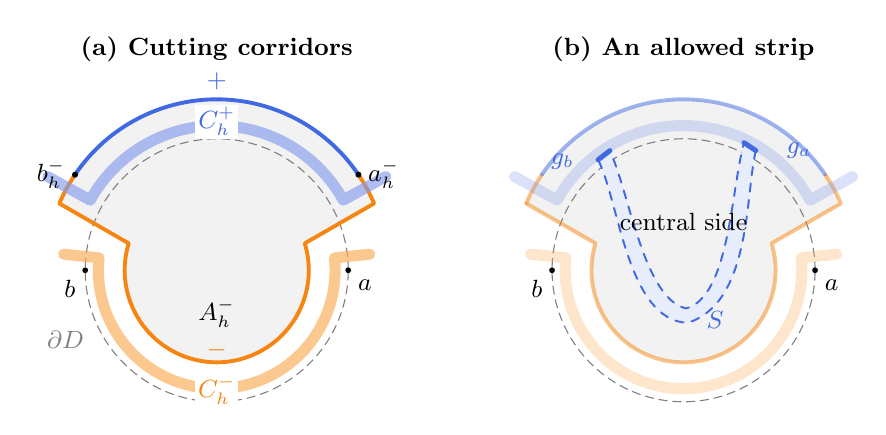
\begin{tikzpicture}[scale=1.67,line cap=round,line join=round,
  every node/.style={font=\small},
  plus/.style={draw=RoyalBlue,line width=1.4pt},
  minus/.style={draw=BurntOrange,line width=1.4pt},
  cutplus/.style={draw=RoyalBlue!65,line width=4pt,opacity=.65},
  cutminus/.style={draw=BurntOrange!65,line width=4pt,opacity=.65}]
\begin{scope}
  \node[font=\small\bfseries] at (0,1.68) {(a) Cutting corridors};
  \fill[gray!10] (23:1.30) arc[start angle=23,end angle=157,radius=1.30]
    -- (163:.70) arc[start angle=163,end angle=377,radius=.70] -- cycle;
  \draw[densely dashed,gray] (0,0) circle[radius=1];
  \draw[minus] (157:1.30)--(163:.70)
    arc[start angle=163,end angle=377,radius=.70]--(23:1.30)
    arc[start angle=23,end angle=34,radius=1.30];
  \draw[minus] (146:1.30) arc[start angle=146,end angle=157,radius=1.30];
  \draw[plus] (34:1.30) arc[start angle=34,end angle=146,radius=1.30];
  \draw[cutplus] (29:1.47)--(29:1.10)
    arc[start angle=29,end angle=151,radius=1.10]--(151:1.47);
  \draw[cutminus] (174:1.17)--(174:.90)
    arc[start angle=174,end angle=366,radius=.90]--(366:1.17);
  \node[RoyalBlue,fill=white,inner sep=1pt] at (0,1.13) {$C_h^+$};
  \node[BurntOrange,fill=white,inner sep=1pt] at (0,-.91) {$C_h^-$};
  \node at (0,-.33) {$A_h^-$};
  \node[gray] at (-1.15,-.53) {$\partial D$};
  \fill (1,0) circle[radius=.022] node[below right] {$a$};
  \fill (-1,0) circle[radius=.022] node[below left] {$b$};
  \fill (34:1.30) circle[radius=.023] node[right] {$a_h^-$};
  \fill (146:1.30) circle[radius=.023] node[left] {$b_h^-$};
  \node[RoyalBlue] at (0,1.44) {$+$};
  \node[BurntOrange] at (0,-.61) {$-$};
\end{scope}
\begin{scope}[xshift=3.55cm]
  \node[font=\small\bfseries] at (0,1.68) {(b) An allowed strip};
  \fill[gray!10] (23:1.30) arc[start angle=23,end angle=157,radius=1.30]
    -- (163:.70) arc[start angle=163,end angle=377,radius=.70] -- cycle;
  \draw[densely dashed,gray] (0,0) circle[radius=1];
  \draw[minus,opacity=.5] (157:1.30)--(163:.70)
    arc[start angle=163,end angle=377,radius=.70]--(23:1.30)
    arc[start angle=23,end angle=34,radius=1.30];
  \draw[minus,opacity=.5] (146:1.30) arc[start angle=146,end angle=157,radius=1.30];
  \draw[plus,opacity=.5] (34:1.30) arc[start angle=34,end angle=146,radius=1.30];
  \draw[cutplus,opacity=.3] (29:1.47)--(29:1.10)
    arc[start angle=29,end angle=151,radius=1.10]--(151:1.47);
  \draw[cutminus,opacity=.3] (174:1.17)--(174:.90)
    arc[start angle=174,end angle=366,radius=.90]--(366:1.17);
  \path[fill=RoyalBlue!12,draw=RoyalBlue,dashed,line width=.7pt]
    (.55,.91)..controls (.47,.60) and (.52,-.25)..(.03,-.40)
    ..controls (-.43,-.38) and (-.49,.53)..(-.65,.84)
    --(-.56,.91)
    ..controls (-.41,.58) and (-.30,-.22)..(.02,-.29)
    ..controls (.35,-.20) and (.36,.61)..(.46,.97)--cycle;
  \draw[plus,line width=1.8pt] (.55,.91)--(.46,.97);
  \draw[plus,line width=1.8pt] (-.65,.84)--(-.56,.91);
  \node[RoyalBlue] at (.88,.91) {$g_a$};
  \node[RoyalBlue] at (-.92,.83) {$g_b$};
  \node[RoyalBlue] at (.24,-.38) {$S$};
  \node at (0,.37) {central side};
  \fill (1,0) circle[radius=.022] node[below right] {$a$};
  \fill (-1,0) circle[radius=.022] node[below left] {$b$};
\end{scope}
\end{tikzpicture}

 \caption{Schematic geometry in Schoenflies coordinates for the
 minus-favoring comparison.  The dashed circle represents
 $\partial D$.  The boundary of $A_h^-$ is enlarged along its middle
 plus arc and moved inward elsewhere.  The blue cutting corridor is
 outside $D$; its caps cross the minus shoulders of $A_h^-$.  The
 orange corridor is outside $A_h^-$ and cuts off the target minus
 arc.  In the second panel an allowed plus strip lies on the central
 side of both cuts, with gates outside $D$.  Widths and displacements
 are exaggerated.  The strip is a deterministic test region, not a
 sampled interface, and the physical construction uses polygonal
 approximations.}
 \label{fig:strip-squeeze}
\end{figure}

At each fixed $h$ these placements are valid for every sufficiently
large $n$.  Boundary winding controls the compact clearances, and the
marked boundary order controls signs near each contact.  The caps
prevent paths from going around the ends of a cut.  This remains true
for a free path ending next to an exterior pin: append its final
incident bond before applying separation.  With pinned boundary
vertices that last bond already lies in the polygon.  The difference
between the two conventions is contained in one lattice layer and
cannot defeat a fixed-clearance cap.

\subsection{Conditioning at a fixed environment}

For laws of vectors in $\{0,1\}^m$, write $\preceq$ for stochastic
order with respect to coordinatewise order.  We record the elementary
coupling fact from \cite[Section~9, Lemma ``Conditioning and gluing at
fixed environment'']{R}, including its proof because its conditional
marginal is essential here.

\begin{lemma}[Conditional gluing]
\label{lem:conditional-gluing}
Let $\lambda$ be a deterministic law on a finite set and $\mu_\omega$
a measurable environmental family of laws on another finite set.
Let $U,W$ be vector-valued functions on these sets with values in
$\{0,1\}^m$.  Suppose $p,q_\omega$ are laws of
$(e,v)\in\{0,1\}\times\{0,1\}^m$, with $q_\omega$ measurable,
$p$ deterministic, and
$p(e=1)\ge c>0$, such that
\[
 \mathcal L_\lambda(U)\preceq p(v\in\cdot\mid e=1),\qquad
 q_\omega(v\in\cdot\mid e=1)\preceq\mathcal L_{\mu_\omega}(W)
\]
whenever the second conditional law is defined.  There is a measurable
coupling $\pi_\omega$ of $\lambda,\mu_\omega$ satisfying
\[
 \E_{\rm env}\pi_\omega\{U\npreceq W\}
 \le \frac{6}{c}\E_{\rm env}\|p-q_\omega\|_{\TV}.
\]
In particular its first marginal is $\lambda$ in every environment.
\end{lemma}

\begin{proof}
Put $e_\omega=\|p-q_\omega\|_{\TV}$.  On $e_\omega\le c/2$,
$q_\omega(e=1)\ge c/2$, and subtraction of the conditional fractions
gives
\[
 \|p(v\in\cdot\mid e=1)-q_\omega(v\in\cdot\mid e=1)\|_{\TV}
 \le 4e_\omega/c.
\]
Couple these middle vectors maximally and glue to the two order
couplings.  Extend the outer vectors to complete samples using their
conditional laws given $U,W$.  Order fails only when the middle
vectors disagree.  On $e_\omega>c/2$ use any coupling with the same
prescribed marginals; this exceptional set has probability at most
$2\E_{\rm env}e_\omega/c$.  This proves the bound.  All required
couplings are measurable finite-dimensional kernels: enumerate the
finitely many linear-programming bases of each coupling problem and
select the first feasible basic solution.  Subsequent conditional
probabilities are explicit finite ratios, with a fixed arbitrary
probability law on each zero-mass fiber.
\end{proof}

The environment has not been conditioned on $e=1$.  We condition spin
laws separately at each fixed environment, including when deciding
which environments require an arbitrary coupling.

\begin{proposition}[Transfer of a finite strip family]
\label{prop:strip-transfer}
Fix $h>0$ and a finite family of allowed plus strips in $A_h^-$.
The pure critical Dobrushin sample in an ordinary mesh approximation
of $A_h^-$ and the target sample in $D_n$ admit couplings conditional
on the original environment such that every strip crossed by plus in
the pure sample is crossed by plus in the virtually filled target,
with annealed probability $1-o(1)$.  The pure marginal conditional on
the original environment is its deterministic pure law.  The analogous
assertion holds for minus strips in $A_h^+$.
\end{proposition}

\begin{proof}
Embed the target and comparison domains, their incident bond layers,
the two corridors, their reveal regions, and the strips in a torus
chart with a fixed positive buffer.  Use the target bond
environment in that chart and independent bonds to complete the
torus, whose period is chosen as in Proposition~\ref{prop:torus-tests}.
Until the final averaging step include those extra bonds in the environment.
Let $E_h$ be the event of the two required cutting crossings, and
$V$ the vector of ordinary plus strip crossings in the torus.  For
the pure and quenched torus vector laws $p_n,q_{n,\omega}$,
\begin{equation}
 p_n(E_h)\ge c_h>0,\qquad
 \E_{\rm env}\|p_n-q_{n,\omega}\|_{\TV}\longrightarrow0.
 \label{eq:strip-middle-laws}
\end{equation}
The first assertion is the pure buffered RSW construction for two
disjoint prescribed-color corridors
\cite[Section~2, Proposition ``Pure buffered RSW consequences'']{S};
the second is Proposition~\ref{prop:torus-tests}, applied to the
fixed finite vector $(\1_{E_h},V)$.  No comparison of the entire
torus spin configurations is asserted.

We verify the two stochastic orders needed for
Lemma~\ref{lem:conditional-gluing}.  In either torus conditioned on
$E_h$, inspect each corridor from its exterior side, stopping at its
first crossing of the required color.  The construction is
\cite[Section~6, Lemma ``Reveals with a monochromatic facing
boundary'']{S}.  It can be described by querying the inspecting
boundary and expanding the queried cluster of the opposite color.
Every unqueried neighbor of that cluster is queried; queried vertices
of the required color are not expanded.  On success the facing
boundary is the required monochromatic crossing, and nothing beyond
it toward the center is queried.  Planarity of the triangulation
gives this facing crossing; the cap extensions ensure that every
nearest-neighbor incidence across the explored side meets one of
its pins.  The two reveal regions are disjoint.

For clarity, an adaptive stopped reveal has exactly the required
conditional law.  Its next queried site and its stopping decision are
functions of the preceding answers.  A completed transcript
$(v_1,s_1),\ldots,(v_k,s_k)$ therefore occurs precisely when those
queried spins have those values.  Conditioning on the transcript
pins those spins and imposes no further restriction.  Since the
transcripts determine $E_h$, conditioning on $E_h$ adds nothing once
the transcripts are specified.

In the first comparison, the lower law is pure Dobrushin in $A_h^-$
and the upper law is the pure torus conditioned on $E_h$.  In the
union of the whole common nearest-neighbor free components containing
the strip portions on the central side, the revealed plus path
is an upper plus pin against a lower free site.  It screens the
comparison domain's plus boundary.  All remaining accessible domain
boundary incidences are lower minus pins against upper free sites.
At a meeting they are upper plus against lower minus.  The minus
reveal is outside $A_h^-$.  Thus the pure-domain strip vector is
below $p_n(V\in\cdot\mid E_h)$.

In the second comparison, the lower law is the quenched torus
conditioned on $E_h$ and the upper law is the target.  Again use the
whole common nearest-neighbor free components containing the interior
strip portions on the central side.  Now the minus
path screens the target minus boundary, and the plus reveal is
outside the target.  With the upper entry first, the incidences are
\[
 (+,\mathrm{free}),\qquad (\mathrm{free},-),\qquad (+,-).
\]
All bonds incident to common free vertices have identical couplings
in the two laws being compared.  Condition on the other spins.
Each displayed pair orders the resulting boundary fields, regardless
of the value of a free site in that pair.  The nearest-neighbor
ferromagnetic boundary comparison therefore orders the conditional
spin laws; averaging over these other spins preserves the order.
This argument takes place at fixed environment and uses only
$K_e(\beta_*)>0$.  It does not compare pure bond strengths with
random bond strengths.

The geometric incidence verification is precisely that of
\cite[Section~9, proof of ``Quenched transfer of a finite strip
family'']{R} and \cite[Section~7, proof of ``Fixed-geometry boundary
squeeze'']{S}.  A nearest-neighbor edge cannot cross a triangulated
path in the interior of an edge; the caps prevent an incidence from
escaping around a cut.  The marked clearances established above
exclude a wrongly signed accessible boundary pin.  These statements
also cover the last edge to an exterior pin and the boundary-vertex
convention.  Virtual plus values give the upper value on every
portion of a strip outside $D_n$.  We obtain, jointly for the entire
finite list,
\[
 \mathcal L(V_{A_h^-})\preceq p_n(V\in\cdot\mid E_h),\qquad
 q_{n,\omega}(V\in\cdot\mid E_h)\preceq\mathcal L_\omega(V_{D_n}).
\]
Lemma~\ref{lem:conditional-gluing} and
\eqref{eq:strip-middle-laws} give the result for vector laws and,
by disintegration, for full spin samples.  Average over the added
torus bonds conditional on the original environment.  The target
marginal never used those bonds, and the pure marginal remains its
fixed pure law.  The sign-reversed construction is identical.
\end{proof}

\subsection{From strips to ordered traces}

To use a virtually filled crossing as a barrier, one needs exact
noncrossing, rather than just two drawings at distance $O(\delta_n)$.
We give the boundary check from
\cite[Section~7, Lemma ``Local drawing beside a signed strip'']{S}.
For a fixed finite strip list, its boundary contacts lie on compact
signed arcs separated from the marks.  Near a plus contact every
exterior nearest neighbor of a free site is already plus.  Fill the
other exterior vertices of incident faces with plus for drawing
purposes.  In the cell convention, a boundary dual vertex meets one,
two adjacent, or three interior cells; two opposite cells alone would
violate the Jordan condition.  With one interior cell, the two
nearest exterior neighbors already have the filling sign, so filling
the opposite exterior corner changes no bond incident to that cell.
With two adjacent or three interior cells, all exterior corners are
already nearest neighbors.  Triangular interpolation consequently
preserves every target disagreement edge and every resolved local
connection.  With pinned boundary vertices the same assertion follows
directly by interpolating the plaquettes with their given arc values.

Redraw the target in the faces meeting the strips and one adjacent
layer using these zero segments.  They glue at the same edge
midpoints, preserve traversal order, and avoid all corresponding
monochromatic paths.  Plus and minus contact sets are separated, so
the two fillings can be made simultaneously.  The half-edge ends
and neighborhoods of the marks are untouched.  Denote the resulting
drawing by $\widetilde\Gamma_n$; then
\begin{equation}
 d_{\rm curv}(\widetilde\Gamma_n,\Gamma_n)=O(\delta_n),
 \qquad \widetilde\Gamma_n\text{ is disjoint from every selected barrier}.
 \label{eq:barrier-redrawing}
\end{equation}
This changes the drawing only, including in a domain with narrow
fjords: no exterior spin or incident interaction is removed.

We use the following pure geometric input from
\cite[Section~9, Lemma ``Finite strips and limiting barriers'']{R},
proved in \cite[Section~7, ``From fixed strip tests to limiting
barriers'']{S}.  Given $\eta_j\downarrow0$, one can choose
$h_j\downarrow0$ and a deterministic finite list of allowed strips
of each sign at displacement $h_j$ such that, outside pure
probability $O(\eta_j)$, a comparison chord selects a strip whose
end gates it crosses with strict margins.  Its omitted terminal
pieces have diameter at most $\eta_j$.  The strip has cross-sections
of diameter at most $\eta_j$ following a simple prototype within
$\eta_j$ in curve distance of the remaining subarc.  For sufficiently
fine ordinary lattice approximations the same assertion holds, with
errors $O(\eta_j)$, and the signed side of the lattice interface
supplies a monochromatic crossing of that strip.

Here are the relevant hypotheses and parameter order behind this
input.  The pure Dobrushin convergence to $\SLE_3$ is used only in a
fixed polygonal domain, with the full curve convergence supplied by
\cite{CDHKS,KS}; see also the pure input statements in~\cite{R,S}.
Uniform convergence of Jordan boundary parametrizations gives
uniform convergence on the closed disk of the normalized conformal
maps, by Rad\'o's domain-continuity theorem as stated and explained
in~\cite[Section~7, beginning of ``From fixed strip tests to limiting
barriers'']{S}.  In particular the hypotheses give a common boundary
local-connectedness modulus.  Uniform convergence transfers nearby
points on the varying boundaries to nearby points of the limiting
boundary; uniform continuity of the limiting inverse and of the
parametrizations then controls a joining boundary subarc.  The boundary
crosscut proof of the conformal extension theorem upgrades kernel
convergence using this modulus.  Thus boundary fjords do not require
an extra regularity assumption.  Mapping a single disk
$\SLE_3$ by those maps shows that the continuum laws in $A_h^\pm$
converge in the oriented curve metric to $\SLE_3(D;a,b)$ as
$h\downarrow0$.  Simplicity and avoidance of the boundary away from
the two endpoints imply that compact middle subarcs stay inside $D$.
In the enlarged domain, take the last and first hits of
$\rho=1+h/3$ around an interior point and extend slightly at their
ends.  These hits are on the enlarged signed side, outside $D$;
the extensions stay below $1+h/2$.  Polygonal tolerances are chosen
smaller than the gaps between these radial levels.  This gives the allowed gates,
and the omitted terminal diameters tend to zero.  Thin rectangular
neighborhoods of these simple subarcs can be chosen polygonal with
strict traversal margins.  Rational choices form a countable open
cover of the favorable curves; a finite subcover in probability
loses at most another $\eta_j$.  To see the signed crossing in a fine
lattice approximation, follow the selected interface traversal through
its successive interpolation triangles.  Their plus-side vertices
are connected by plus edges of those triangles, with common vertices
or edges across each consecutive face.  They form a plus walk at
distance $O(\delta_n)$ from the traversal.  The positive long-side
clearance keeps this walk inside the strip; the transverse crossing
margins carry it beyond both end gates.  Crop it at those gates and
erase loops.  Backtracking of the interface does not affect this
existence argument.  The entire finite list is fixed
before Proposition~\ref{prop:strip-transfer} is applied.  The sampled
curve chooses its strip only afterwards.

Choose increasing deterministic integers $n_j\ge j$ so that for
every $n\ge n_j$ all fixed-$j$ placements, pure approximation bounds,
and both strip transfers have errors at most $O(\eta_j)$, and the
pure comparison laws are within $\eta_j$ of their continuum laws in
bounded-Lipschitz distance.  Include the fixed-clearance exterior
closures described below among these requirements.  This absorbs
the possibly small $c_{h_j}$ in the conditional coupling estimate.
Set
\begin{equation}
 j(n)=\max\{j\le n:n_j\le n\}.
 \label{eq:interface-diagonal}
\end{equation}
Before $n_1$ make any choice.  Then $j(n)\to\infty$.
Let $L_n$ be the pure comparison chord in $A_{h_{j(n)}}^-$ and
$U_n$ the pure comparison chord in $A_{h_{j(n)}}^+$, both oriented
from the mark near $a$ to that near $b$.
Glue their couplings over the common pair consisting of the original
environment and target spin sample, by sampling the two conditional
comparison kernels given that pair.  Each comparison marginal
conditional on the original environment remains its deterministic
pure law.  Both marginal laws converge to $\SLE_3(D;a,b)$, and
with probability tending to one the target has both selected barriers.

All target traces eventually lie in a fixed compact planar disk.
The space of its nonempty compact subsets is compact in Hausdorff
distance.  Together with tightness of $L_n,U_n$ in the curve metric,
this gives, along any further subsequence, a joint subsequential limit
\[
 (\operatorname{tr}\Gamma_n,L_n,U_n)\Longrightarrow(K,L,U).
\]
Here $K$ is connected, contains $a,b$, and lies in $\overline D$;
these facts follow respectively from Hausdorff convergence,
endpoint convergence, and the boundary winding argument.
Both $L,U$ are simple $\SLE_3$ chords with interiors in $D$.
For such a chord $C$, let $P(C),M(C)$ denote the open components of
$D\setminus C$ adjacent to $I_+,I_-$, respectively.

The barriers imply
\begin{equation}
 K\subset\overline{M(L)}\cap\overline{P(U)},
 \label{eq:trace-squeeze}
\end{equation}
where closures are in $\overline D$.  We spell out why this includes
the open boundary arcs, following
\cite[Section~7, ``Forbidden sides, order, and identification of the
trace'']{S}.  Represent the subsequential convergence almost surely
and, after a further subsequence, make barrier failures summable.
Erase loops in a successful plus crossing, join its ends to the gate
centers within the exterior gate neighborhoods, and close it by
radial paths in $\Psi$ coordinates to a fixed circle $\rho=\rho_*>1$,
followed by its plus-side circular arc.  The added paths have positive
clearance from $\overline D$ at each fixed $j$; the thresholds $n_j$
ensure that they are outside $D_n$.  Both target marks are on the
zero-winding side: their outward escape paths lie beyond the ends
of the extended plus arc.  Exact disjointness in
\eqref{eq:barrier-redrawing} keeps the entire target on that side.

The closed path need not be simple; its winding number is constant
along any curve disjoint from it.  Every crossing between the strip gates is homotopic within the
rectangular strip, relative to its gates, to its prototype.  Thus
backtracking of that crossing cannot alter its winding about points
outside the strip.  Vanishing strip widths, prototype errors, and
terminal diameters make this winding equal eventually to the nonzero
winding of $L$ closed on the plus side, on each compact subset of
$P(L)$.  The fixed outer circular arc remains a positive distance
beyond each compact subarc of $I_+$, and the connectors tend to the
two endpoint connectors.  The same nonzero winding therefore holds
in a neighborhood of every point of $I_+$ other than $a,b$.
The target avoids all these neighborhoods.  Its limit lies in
$\overline{M(L)}$, and the minus barrier gives the other inclusion
in~\eqref{eq:trace-squeeze}.

\begin{lemma}[Ordered chords with equal laws]
\label{lem:ordered-chords}
Let $L,U$ be random simple chords from $a$ to $b$ with interiors in
$D$, and let $K\subset\overline D$ be random, compact, connected,
and contain $a,b$.  If \eqref{eq:trace-squeeze} holds, then
$P(L)\subset P(U)$ almost surely.  If $L,U$ have the same trace law,
then $K=L=U$ as compact sets almost surely.
\end{lemma}

\begin{proof}
This elementary planar argument is
\cite[Section~7, Lemma ``Ordered chords with equal laws'']{S}.
If $P(L)\cap M(U)$ were nonempty, a point in the intersection could
be joined inside these side domains to the two opposite open boundary
arcs.  Removing loops gives a crosscut between those arcs disjoint
from $K$, by~\eqref{eq:trace-squeeze}.  Its endpoints alternate
with $a,b$, so it separates $a$ from $b$, contradicting connectedness.
Thus $P(L)\subset P(U)\cup U$.  An interior point of $U$ cannot
lie in the open set $P(L)$, because every neighborhood of that point
meets $M(U)$.  Hence $P(L)\subset P(U)$.

Map to the disk by the fixed Schoenflies map and take the ordinary
areas of the two plus sides.  These bounded random variables are
ordered and have the same distribution, so their difference is zero
almost surely.  A proper inclusion of the side domains would give
positive area difference: a point in $P(U)\setminus P(L)$ is either
in $M(L)$, or on $L$, in which case its neighborhood in $P(U)$ meets
$M(L)$.  The difference therefore contains a nonempty open set.
The plus sides, and hence their interior boundary chords, are equal.
Finally \eqref{eq:trace-squeeze} puts $K$ on that chord.  Its inverse
parametrization sends $K$ to a connected subset of $[0,1]$ containing
both endpoints, necessarily all of $[0,1]$.  No zero-area assertion
about the chords was needed.
\end{proof}

Consequently every joint trace limit satisfies $K=L=U$.  It remains
to rule out repeated forward and backward traversal near this trace.

\subsection{Passages control traversal order}

The passage criterion below is proved in
\cite[Section~7, Lemma ``Progress coordinates and the full curve
metric'']{S}; we include its proof to make the passage from compact
sets to oriented curves explicit.  It uses the interior estimate
of Corollary~\ref{cor:four-passages}.  This is a concrete version
of the role of multiple-crossing bounds in curve compactness
arguments~\cite{AB,KS}.

\begin{lemma}[Progress along a simple limiting chord]
\label{lem:progress}
Suppose $g_n$ are simple oriented curves, their endpoints tend to
$a,b$, and their traces converge in Hausdorff distance to that of
an injective continuous chord $G:[0,1]\to\overline D$ with endpoints
$a,b$ and $G((0,1))\subset D$.  There are continuous
$u_n:[0,1]\to[0,1]$, with endpoint values tending to $0,1$, such that
\[
 e_n:=\sup_t|g_n(t)-G(u_n(t))|\longrightarrow0.
\]
If $B_n:=\sup_{s<t}(u_n(s)-u_n(t))\to0$, then
$d_{\rm curv}(g_n,G)\to0$.  Conversely, for each $0<\eta<1$,
a drop $B_n\ge\eta$ forces six disjoint passages from radius $r$
to radius $R_\eta>0$ about a point of
$G([\eta/2,1-\eta/2])$, for every $e_n<r<R_\eta$ and all
sufficiently large $n$.  Here $R_\eta$ depends only on $G,\eta$.

The corresponding convergence in probability holds for random
coupled curves if trace and endpoint convergence hold in probability
and, for every deterministic $F\Subset D$ and all sufficiently small
fixed $R>0$,
\begin{equation}
 \lim_{r\downarrow0}\limsup_n
 \Prob\{g_n\text{ has four passages from }r\text{ to }R
                     \text{ about some point of }F\}=0.
 \label{eq:progress-passage}
\end{equation}
Passages are counted on disjoint open parameter intervals.
\end{lemma}

\begin{proof}
Extend the continuous inverse coordinate $G^{-1}$ from its compact
trace continuously to an ambient neighborhood, with values in
$[0,1]$, and compose it with $g_n$.  Uniform continuity gives the
assertions about $u_n,e_n$ and their endpoints.  If $B_n\to0$,
the running maximum $m_n(t)=\max_{s\le t}u_n(s)$ satisfies
$0\le m_n(t)-u_n(t)\le B_n$.  Normalize its endpoint values to
$0,1$, obtaining a nondecreasing continuous $v_n$ with
$\|v_n-u_n\|_\infty\to0$.  For any $\kappa_n\downarrow0$ with
$\kappa_n>0$, the function
$h_n(t)=(1-\kappa_n)v_n(t)+\kappa_n t$ is an increasing
homeomorphism of $[0,1]$.  If $\omega_G$ is the modulus of
continuity of $G$, then
\[
 d_{\rm curv}(g_n,G)
 \le e_n+\omega_G(\|h_n-u_n\|_\infty)\longrightarrow0.
\]

If instead $u_n(s)-u_n(t)\ge\eta$ for some $s<t$, put
$c_n=(u_n(s)+u_n(t))/2\in[\eta/2,1-\eta/2]$.  Once endpoint
coordinate errors are less than $\eta/4$, each of $[0,s],[s,t],[t,1]$
has endpoints on opposite sides of $c_n$, at coordinate distance
at least $\eta/4$.  Each interval contains a visit to $c_n$.
Injectivity and compactness give
\[
 q_\eta=\min_{|v-w|\ge\eta/4}|G(v)-G(w)|>0,\qquad
 d_\eta=\dist(G([\eta/2,1-\eta/2]),\partial D)>0.
\]
Choose $R_\eta<\min(q_\eta,d_\eta)/4$.  For $e_n<R_\eta$,
the four anchor points at parameters $0,s,t,1$ are outside the
radius-$R_\eta$ disk about $G(c_n)$, whereas the three level visits
are within $e_n$ of its center.  Cropping the incoming and outgoing
pieces at the inner and outer hits gives two annular passages in
each interval.  Their open parameter intervals are disjoint, and
simplicity makes their spatial interiors disjoint.  Thus there are
six passages, in particular four.  Fixed-factor crops give the same
conclusion for square annuli if those are used in
Corollary~\ref{cor:four-passages}.

For the random assertion, use a measurable continuous representative
of $G$.  Measurable progress coordinates are obtained without choosing
a random extension: write
$\Delta_n=d_H(\operatorname{tr}g_n,\operatorname{tr}G)$,
$z_n=2\Delta_n+1/n$, and set
\[
 u_n(t)=
 \frac{\displaystyle\int_0^1 v\,(z_n-|g_n(t)-G(v)|)_+\,\dd v}
 {\displaystyle\int_0^1 (z_n-|g_n(t)-G(v)|)_+\,\dd v}.
\]
The denominator is positive, and this is continuous in $t$ and
jointly measurable.  Put
$\iota_G(r)=\sup\{|v-w|:|G(v)-G(w)|\le r\}$, which tends to
zero with $r$.  Parameters receiving positive weight have diameter
at most $\iota_G(2z_n)$, so
\[
 e_n\le z_n+\omega_G(\iota_G(2z_n))\longrightarrow0
\]
in probability; endpoint coordinate errors also tend to zero.
These statements follow almost surely along any subsequence on
which the trace and endpoint errors converge almost surely, and
hence in probability for the full sequence.

Fix $\eta>0$ and an exceptional probability $\zeta>0$.  Choose
deterministic $q,d>0$ with
$\Prob(q_\eta<q\text{ or }d_\eta<d)<\zeta$.  The random
centers then lie in the deterministic compact set
$F_d=\{z\in\overline D:\dist(z,\partial D)\ge d\}$.
Fix a deterministic $R<\min(q,d)/8$ small enough for
\eqref{eq:progress-passage}.  For every fixed $0<r<R$, the
six-passage argument bounds
\[
 \limsup_n\Prob(B_n\ge\eta)
 \le \zeta+\limsup_n\Prob\{\text{four passages about some point of }
                                      F_d\text{ from }r\text{ to }R\}.
\]
Let $r\downarrow0$ and then $\zeta\downarrow0$.  Thus
$B_n\to0$ in probability.  Localizing the random continuity
modulus $\omega_G$ outside another event of probability $\zeta$
and using the running-maximum construction gives the asserted
curve convergence.  All compact sets and radii used in the passage
estimate are deterministic before taking the mesh limit.
\end{proof}

\subsection{Completion of the main theorem}

\begin{proof}[Proof of Theorem~\ref{thm:main}]
The tuning, matching, and criticality arguments give
$\beta_* =\beta_c^\rho(\varepsilon)$ for all sufficiently small
fixed $\varepsilon>0$.  The tuning estimate
$\beta_*=K_0+O_\rho(\varepsilon^2)$ also gives the critical-temperature
estimate in the theorem.  Choose $\varepsilon_0(\rho)$ once to meet
their smallness conditions and the fixed-shape crossing bootstrap.
These choices precede every final domain, strip family, and
approximation sequence.

Begin with any subsequence of the deterministic approximations, and
pass further to fix the signed arc designation.  The slow diagonal
\eqref{eq:interface-diagonal} constructs couplings of the target and
two comparison chords satisfying
\[
 \mathcal L(\Gamma_n\mid\omega)=Q_{n,\omega},\qquad
 \mathcal L(L_n\mid\omega)=R_n,
 \qquad R_n\Longrightarrow\SLE_3(D;a,b),
\]
where $R_n$ is deterministic.  Every further subsequence has a joint
trace and comparison-curve limit, and the barrier argument and
Lemma~\ref{lem:ordered-chords} identify it as $(L,L,L)$ in traces.

We explain the probabilistic passage to curves without assuming
target curve tightness.  The space of continuous oriented curves
modulo zero uniform reparametrization distance is Polish.  Rational
polygonal paths are dense.  For completeness, select a Cauchy
subsequence with successive distances less than $2^{-j}$, choose
parametrized representatives $g_j$, and put $f_1=g_1$.  Given a
fixed representative $f_j$, choose increasing homeomorphisms
$\alpha,\beta$ such that
$\|f_j\circ\alpha-g_{j+1}\circ\beta\|_\infty<2^{1-j}$, and put
$f_{j+1}=g_{j+1}\circ\beta\circ\alpha^{-1}$.  Then
$\|f_{j+1}-f_j\|_\infty<2^{1-j}$.  The representatives converge
uniformly to a continuous path $f$, and
$d_{\rm curv}(f_j,f)\le\|f_j-f\|_\infty\to0$; the original
Cauchy sequence has the same limit.  Pauses are permitted in this
ambient continuous-curve space and removed by the zero-distance
identification when appropriate.  Thus the joint trace and comparison
convergence admits an almost surely convergent representation.
Lift that representation to target paths by their original
conditional laws given the trace and the two comparison curves.
At each mesh the target has finite configuration space, so these
kernels exist directly.  The lift preserves every joint law at
that mesh, and in particular every annealed target passage bound.

Corollary~\ref{cor:four-passages} gives
\eqref{eq:progress-passage} for these target curves: interior
charts have fixed free buffers, arbitrary exterior spins are allowed,
and target passages are bounded by the local event that any resolved
contours supply the required passages.  Local redrawings are absorbed
by fixed-factor radius crops.  Lemma~\ref{lem:progress} now gives
$d_{\rm curv}(\Gamma_n,L)\to0$ in probability in the representation.
Since also $L_n\to L$ in curve distance,
$d_{\rm curv}(\Gamma_n,L_n)\to0$ there and hence in the original
couplings.  Every further subsequence permits this argument, so it
holds along the chosen sequence.  In particular
\begin{equation}
 \E\min\{1,d_{\rm curv}(\Gamma_n,L_n)\}\longrightarrow0.
 \label{eq:quenched-coupling-error}
\end{equation}

Write $\bar d=\min\{1,d_{\rm curv}\}$.  For any test function
in the bounded-Lipschitz class for $\bar d$, the conditional coupling
and its two correct marginals give
\[
 \left|\int F\,\dd Q_{n,\omega}-\int F\,\dd R_n\right|
 \le \E\bigl[\bar d(\Gamma_n,L_n)\mid\omega\bigr].
\]
Taking the supremum over that class and then environmental expectation,
\begin{equation}
 \E_{\rm env}d_{\rm BL}(Q_{n,\omega},R_n)
 \le \E\bar d(\Gamma_n,L_n)\longrightarrow0.
 \label{eq:quenched-bl}
\end{equation}
The conditional pure marginal is essential in this step.  Measurability
holds also for a nonatomic bond law: at each mesh $Q_{n,\omega}$ has
a fixed finite curve support and measurable probabilities, and its
distance to a fixed law is a continuous function of these probabilities.
Added torus bonds and auxiliary coupling variables have already been
integrated out conditional on the original environment.

The deterministic laws $R_n$ converge in bounded-Lipschitz distance
to the stated SLE law.  Equation~\eqref{eq:quenched-bl}, the triangle
inequality, and Markov's inequality prove convergence in environmental
probability on the chosen subsequence.  If it failed for the original
sequence, a subsequence on which the failure probability stayed
positive would contradict this construction.  Finally restore the
prescribed lattice drawing and half-edges; their matched displacement
is $O(\delta_n)$, with the same orientation.  This proves the theorem
in the required uniform oriented-curve metric.
\end{proof}

\begingroup
\raggedright
\begin{thebibliography}{99}
\bibitem{AB}
M.~Aizenman and A.~Burchard,
\emph{H\"older regularity and dimension bounds for random curves},
Duke Math. J. \textbf{99} (1999), 419--453.
\href{https://doi.org/10.1215/S0012-7094-99-09914-3}{doi:10.1215/S0012-7094-99-09914-3}.

\bibitem{AM}
E.~Av\'erous and R.~Mahfouf,
\emph{The near-critical random bond FK-percolation model},
preprint (2025), \href{https://arxiv.org/abs/2509.08938v1}{arXiv:2509.08938v1}.

\bibitem{BS}
A.~I.~Bugrij and V.~N.~Shadura,
\emph{Duality of a two-dimensional nonhomogeneous Ising model on a finite lattice},
Phys. Rev. B \textbf{55} (1997), 11045--11049.
\href{https://doi.org/10.1103/PhysRevB.55.11045}{doi:10.1103/PhysRevB.55.11045}.
Equation locators refer to the preprint
\emph{Duality of the 2D Nonhomogeneous Ising Model on the Torus},
\href{https://arxiv.org/abs/hep-th/9703037v1}{arXiv:hep-th/9703037v1}.

\bibitem{ChayesShtengel}
L.~Chayes and K.~Shtengel,
\emph{Critical behavior for 2D uniform and disordered ferromagnets at self-dual points},
Comm. Math. Phys. \textbf{204} (1999), 353--366.
\href{https://doi.org/10.1007/s002200050649}{doi:10.1007/s002200050649}.
Theorem locators refer to \href{https://arxiv.org/abs/cond-mat/9811203v1}{arXiv:cond-mat/9811203v1}.

\bibitem{CDHKS}
D.~Chelkak, H.~Duminil-Copin, C.~Hongler, A.~Kemppainen, and S.~Smirnov,
\emph{Convergence of Ising interfaces to Schramm's SLE curves},
C. R. Math. Acad. Sci. Paris \textbf{352} (2014), 157--161.
\href{https://doi.org/10.1016/j.crma.2013.12.002}{doi:10.1016/j.crma.2013.12.002}.
Theorem locators refer to \href{https://arxiv.org/abs/1312.0533v2}{arXiv:1312.0533v2}.

\bibitem{ChelkakSmirnov}
D.~Chelkak and S.~Smirnov,
\emph{Universality in the 2D Ising model and conformal invariance of fermionic observables},
Invent. Math. \textbf{189} (2012), 515--580.
\href{https://doi.org/10.1007/s00222-011-0371-2}{doi:10.1007/s00222-011-0371-2}.

\bibitem{DD}
Vik.~S.~Dotsenko and Vl.~S.~Dotsenko,
\emph{Critical behaviour of the 2D Ising model with impurity bonds},
J. Phys. C: Solid State Phys. \textbf{15} (1982), 495--507.
\href{https://doi.org/10.1088/0022-3719/15/3/015}{doi:10.1088/0022-3719/15/3/015}.

\bibitem{DDReview}
Vik.~S.~Dotsenko and Vl.~S.~Dotsenko,
\emph{Critical behaviour of the phase transition in the 2D Ising model with impurities},
Adv. Phys. \textbf{32} (1983), 129--172.
\href{https://doi.org/10.1080/00018738300101541}{doi:10.1080/00018738300101541}.

\bibitem{DCRT}
H.~Duminil-Copin, A.~Raoufi, and V.~Tassion,
\emph{Sharp phase transition for the random-cluster and Potts models via decision trees},
Ann. of Math. (2) \textbf{189} (2019), 75--99.
\href{https://doi.org/10.4007/annals.2019.189.1.2}{doi:10.4007/\allowbreak annals.2019.189.1.2}.
Locators refer to \href{https://arxiv.org/abs/1705.03104v2}{arXiv:1705.03104v2}.

\bibitem{ES}
R.~G.~Edwards and A.~D.~Sokal,
\emph{Generalization of the Fortuin--Kasteleyn--Swendsen--Wang representation and Monte Carlo algorithm},
Phys. Rev. D \textbf{38} (1988), 2009--2012.
\href{https://doi.org/10.1103/PhysRevD.38.2009}{doi:10.1103/PhysRevD.38.2009}.

\bibitem{FK}
C.~M.~Fortuin and P.~W.~Kasteleyn,
\emph{On the random-cluster model. I. Introduction and relation to other models},
Physica \textbf{57} (1972), 536--564.
\href{https://doi.org/10.1016/0031-8914(72)90045-6}{doi:10.1016/0031-8914(72)90045-6}.

\bibitem{FKG}
C.~M.~Fortuin, P.~W.~Kasteleyn, and J.~Ginibre,
\emph{Correlation inequalities on some partially ordered sets},
Comm. Math. Phys. \textbf{22} (1971), 89--103.
\href{https://doi.org/10.1007/BF01651330}{doi:10.1007/BF01651330}.

\bibitem{GGM}
A.~Giuliani, R.~L.~Greenblatt, and V.~Mastropietro,
\emph{The scaling limit of the energy correlations in non-integrable Ising models},
J. Math. Phys. \textbf{53} (2012), 095214.
\href{https://doi.org/10.1063/1.4745910}{doi:10.1063/1.4745910}.
Theorem locators refer to \href{https://arxiv.org/abs/1204.4040v1}{arXiv:1204.4040v1}.

\bibitem{GP}
R.~L.~Greenblatt and E.~Peltola,
\emph{On the spin interface distribution for non-integrable variants of the two-dimensional Ising model},
preprint (2024), \href{https://arxiv.org/abs/2404.12375v3}{arXiv:2404.12375v3}, October 17, 2024.

\bibitem{Harris}
A.~B.~Harris,
\emph{Effect of random defects on the critical behaviour of Ising models},
J. Phys. C: Solid State Phys. \textbf{7} (1974), 1671--1692.
\href{https://doi.org/10.1088/0022-3719/7/9/009}{doi:10.1088/0022-3719/7/9/009}.

\bibitem{Jug}
G.~Jug,
\emph{Critical singularities of the random two-dimensional Ising model},
Phys. Rev. B \textbf{27} (1983), 4518(R).
\href{https://doi.org/10.1103/PhysRevB.27.4518}{doi:10.1103/PhysRevB.27.4518}.

\bibitem{KS}
A.~Kemppainen and S.~Smirnov,
\emph{Random curves, scaling limits and Loewner evolutions},
Ann. Probab. \textbf{45} (2017), 698--779.
\href{https://doi.org/10.1214/15-AOP1074}{doi:10.1214/15-AOP1074}.

\bibitem{KW}
H.~A.~Kramers and G.~H.~Wannier,
\emph{Statistics of the two-dimensional ferromagnet. Part I},
Phys. Rev. \textbf{60} (1941), 252--262.
\href{https://doi.org/10.1103/PhysRev.60.252}{doi:10.1103/PhysRev.60.252}.

\bibitem{Ludwig}
A.~W.~W.~Ludwig,
\emph{Critical behavior of the two-dimensional random $q$-state Potts model by expansion in $(q-2)$},
Nucl. Phys. B \textbf{285} (1987), 97--142.
\href{https://doi.org/10.1016/0550-3213(87)90330-0}{doi:10.1016/0550-3213(87)90330-0}.

\bibitem{Mahfouf}
R.~Mahfouf,
\emph{The near critical random bond Ising model via embedding deformation},
preprint (2025), \href{https://arxiv.org/abs/2509.08928v1}{arXiv:2509.08928v1}.

\bibitem{OSSS}
R.~O'Donnell, M.~Saks, O.~Schramm, and R.~A.~Servedio,
\emph{Every decision tree has an influential variable},
in Proceedings of the 46th Annual IEEE Symposium on Foundations of Computer Science,
IEEE (2005), 31--39.
\href{https://doi.org/10.1109/SFCS.2005.34}{doi:10.1109/SFCS.2005.34}.

\bibitem{R}
OpenAI,
\emph{Quenched $\mathrm{SLE}_3$ Universality for the Weak Random-Bond Ising Model},
OpenAI Math Release preprint
\href{https://github.com/openai/math/blob/main/preprints/Quenched-SLE3-Universality-for-the-Weak-Random-Bond-Ising-Model-October-5-2026/quenched-sle3-weak-random-bond-ising.pdf}{OAI:Quenched-SLE3-Universality-for-the-Weak-Random-Bond-Ising-Model-October-5-2026},
2026.

\bibitem{S}
OpenAI,
\emph{$\mathrm{SLE}_3$ universality for weak finite-range Ising interactions},
OpenAI Math Release preprint
\href{https://github.com/openai/math/blob/main/preprints/SLE3-universality-for-weak-finite-range-Ising-interactions-September-23-2026/paper.pdf}{OAI:SLE3-universality-for-weak-finite-range-Ising-interactions-September-23-2026},
2026.

\bibitem{Schramm}
O.~Schramm,
\emph{Scaling limits of loop-erased random walks and uniform spanning trees},
Israel J. Math. \textbf{118} (2000), 221--288.
\href{https://doi.org/10.1007/BF02803524}{doi:10.1007/BF02803524}.

\bibitem{Shalaev}
B.~N.~Shalaev,
\emph{Correlation function and susceptibility of the two-dimensional Ising model with impurities},
Sov. Phys. Solid State \textbf{26} (1984), 1811--1813;
Russian original, Fiz. Tverd. Tela \textbf{26} (1984), 3002--3005.

\bibitem{Shankar}
R.~Shankar,
\emph{Exact critical behavior of a random bond two-dimensional Ising model},
Phys. Rev. Lett. \textbf{58} (1987), 2466--2469;
erratum, \textbf{59} (1987), 380.
\href{https://doi.org/10.1103/PhysRevLett.58.2466}{doi:10.1103/PhysRevLett.58.2466};
\href{https://doi.org/10.1103/PhysRevLett.59.380.2}{doi:10.1103/PhysRevLett.59.380.2}.

\bibitem{SS}
S.~Sheffield and N.~Sun,
\emph{Strong path convergence from Loewner driving function convergence},
Ann. Probab. \textbf{40} (2012), 578--610.
\href{https://doi.org/10.1214/10-AOP627}{doi:10.1214/10-AOP627}.

\bibitem{Smirnov}
S.~Smirnov,
\emph{Conformal invariance in random cluster models. I. Holomorphic fermions in the Ising model},
Ann. of Math. (2) \textbf{172} (2010), 1435--1467.
\href{https://doi.org/10.4007/annals.2010.172.1435}{doi:10.4007/annals.2010.172.1435}.

\end{thebibliography}
\endgroup

\end{document}
